\pagestyle{fancy}
\fancyhf{}
\renewcommand{\headrulewidth}{0pt}
\fancyfoot[C]{\leftmark}
\fancyhead[R]{\thepage}
\doublespacing
\chapter{Introduction}\label{chap1}

Glasses are one of the most widely used materials in our day-to-day life, due to many dynamic and thermodynamic properties which are very different to many other materials. Some important examples of glasses are silicate glass in the form of window glass, volcanic rocks, metallic glasses, polymeric materials, colloidal glasses, jammed biological assemblies, etc. Fig.~\ref{fig_glassyMaterial} shows the various examples of amorphous solids at different scales, a large part of these materials are glass which ranges from metallic glasses at the nanometer scale to colloidal glasses at micrometer scale \cite{nicolas2018deformation}.  Glassy materials are important ingredients for electronic components, pharmaceutical industry, optical devices, 3-D printing, food processing, etc. These materials have structures very similar to high temperature liquids but the structural relaxation exceeds experimentally available timescales \cite{karmakar2014growing}. Over many decades, scientific investigations \cite{angell1995formation, berthier2011theoretical, binder2011glassy, joshi2018yield,nicolas2018deformation} have continued to understand the hidden information in the structure of glassy materials which lead to ultra slow dynamics where the viscosity of the material becomes $10^{14}$ times the viscosity of the normal liquid, this means effective behaviour as solid. Glassy systems have many unique properties attributed to them: heterogeneous dynamics \cite{karmakar2014growing,garrahan2011dynamic}, change in properties with age (aging) \cite{kob2000fluctuations,abou2001aging}, mechanical memory \cite{keim2019memory,anshul17,fiocco2014encoding}, etc. Although many of these properties have been harnessed for various applications, a deeper understanding of these at the microscopic level would lead to the development of new applications.

    \begin{figure}[hbt!]
	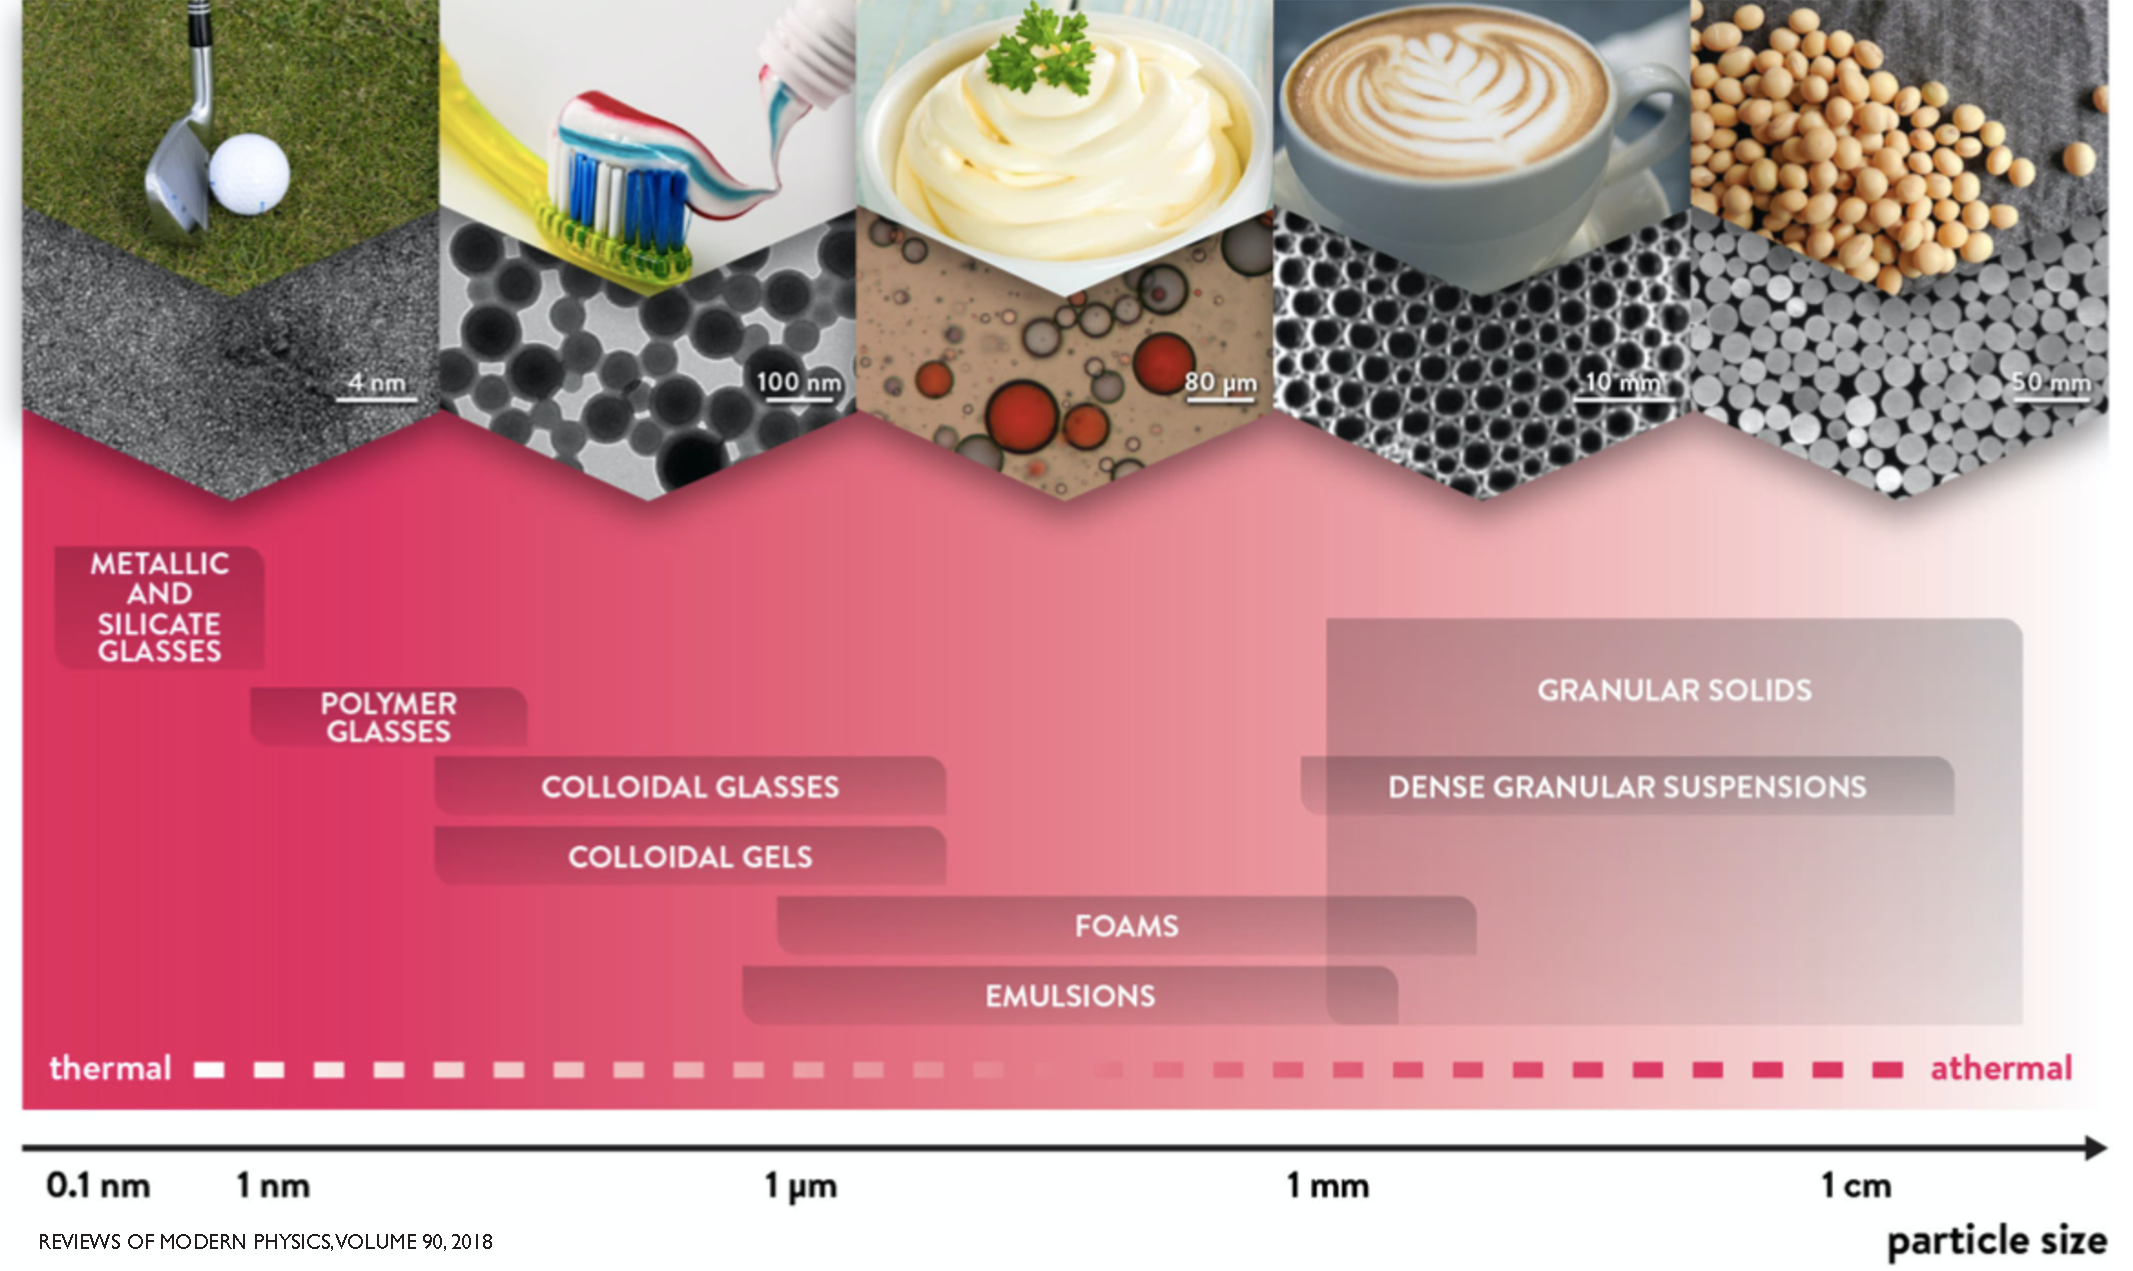
\includegraphics[width=14cm]{figs/glassyMaterial.pdf}
	\centering
	\caption[{\em Schematic representing widespread amorphous materials}]{{\em Schematic representing widespread amorphous materials.} Different amorphous materials found in our day-to-day life have different microscopic scales at their elementary particle level. Schematic adapted from \cite{nicolas2018deformation}.\label{fig_glassyMaterial}}
    \end{figure}

To improve the performance of existing applications and also to develop new applications, it is very important to understand the behaviour of glasses or supercooled liquids under external thermal or mechanical perturbations \cite{keim2019memory,fiocco2014encoding,priezjev2019effect,schuh2007mechanical,hufnagel2015cryogenic}. Such perturbations could be in various forms, but here we are interested in thermal perturbation in the form of a temperature gradient \cite{vaibhav2020response} and mechanical perturbations in the form of shear flow \cite{ludovicRMP2017} and channel flow \cite{vaibhav2021influence,pinaki2014}. Understanding the thermal and mechanical response of glassy systems to such thermal gradient or mechanical deformation will not only allow us to know the non-equilibrium properties of glassy systems but amorphous system, in general. Fig.~\ref{fig_thermoMechanical} shows various examples which highlight the importance of understanding the thermal and mechanical response of glassy systems.

    \begin{figure}[hbt!]
	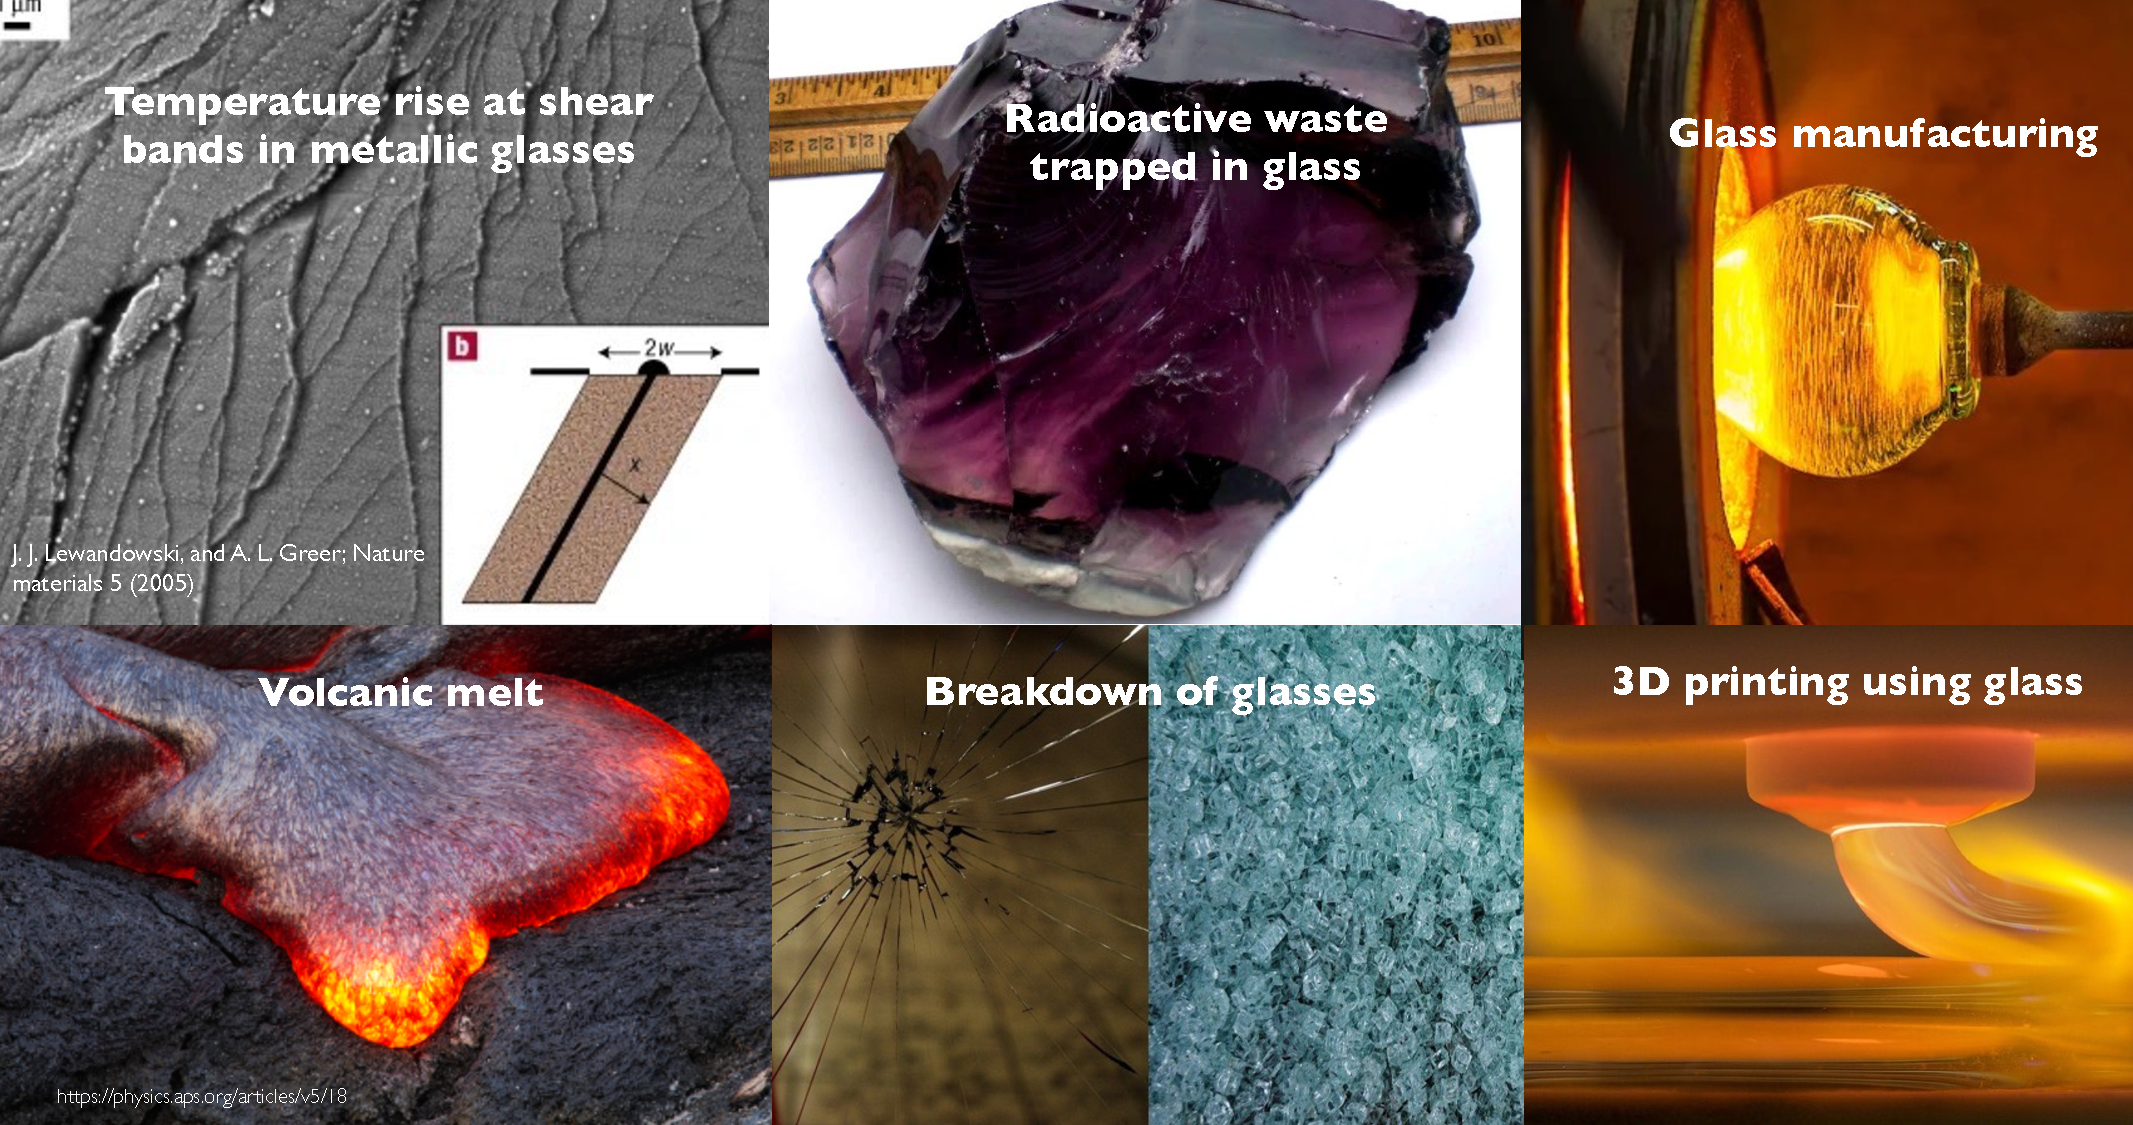
\includegraphics[width=14cm]{figs/thermoMechanical.pdf}
	\centering
	\caption[{\em Importance of thermo-mechanical response of glasses: some examples.}]{{\em Importance of thermo-mechanical response of glasses.} (From top left to right) Local thermal effects due to shear banding in metallic glasses  \cite{lewandowski2006temperature}; Trapping the radioactive nuclear waste in the glass leads to a temperature gradient due to hot nuclear waste leading to possible leakage; Conventional glass manufacturing process involves various heating and cooling protocols. (From bottom left to right) Exposure of extremely hot magma to the environment leads to the inner part of magma being hotter compared to surface resulting in isotope migration and subsequent segregation; Breaking of glass: various applications require improved strength and toughness; 3D printing using glass requires material to flow through a nozzle, like a Poiseuille flow, in a controlled fashion. \label{fig_thermoMechanical}}
    \end{figure}


It is not much known about the response of glassy systems to thermal gradients. Unlike crystalline solids, the mechanism of heat transport in glassy systems is not very clear. Recently, there have been some theoretical attempts to understand heat transport mechanism in crystals and glasses using a unified framework based on Green-Kubo formalism and Boltzmann transport approach \cite{isaeva2019modeling,fiorentino2022green}. The very slow structural relaxation time scales near glass transition present a serious challenge to understand the heat and mass transport properties in glassy systems. Such knowledge is required in trapping nuclear waste materials in glasses \cite{longhurst1985soret,guy1992modelling}, to understand the solidification process of magma coming out of volcanic eruption \cite{koehler2016,dominguez2011soret}, to design thermoresponsive colloids \cite{koniger2013thermophoresis} etc. Therefore, we have pursued the interesting problem of the thermal response of glassy liquids.

Mechanical response of glassy systems is very important to understand to know the failure mechanism under loading and to improve their strength and ductility \cite{schroers2004ductile}, unlike the crystalline systems where defects are the origin of failure \cite{smith1967crack}. Even after the research of the last few decades, there is not a very clear microscopic understanding of the nonlinear flow of such systems \cite{ludovicRMP2017,nicolas2018deformation}. In general, the understanding of emergence of rigidity in glassy materials is important to design new materials with applications. Therefore, investigating the response of glass-forming systems to external mechanical deformation is very interesting. Also, many microfluidic devices, three dimensional printing technology \cite{marchelli2011guide}, memory storage devices, etc. use the flow properties of glassy liquids under confinement. Hence, we have also studied the flow properties of glassy liquid in the Poiseuille flow setup.

At a few occasions, we see that the thermal and mechanical perturbations are present together. For example, during the Poiseuille flow where temperature control is happening via the confining walls \cite{evansMorrissBook}, there is a temperature gradient across the channel. We have also addressed this issue briefly in this thesis. Another form of the possible problem is applying one sort of perturbation after another perturbation. In this context, we have studied a glassy system where a temperature gradient is applied for some finite time to generate some inhomogeneity and then shear response of these inhomogeneous glassy samples is studied.

In the coming sections below, we briefly introduce the supercooled liquids and glasses and also their properties. Following this, a brief introduction to thermal and mechanical response of glasses is presented. In the end, we discuss the organization of this thesis.

%%%%%%%%%%%%%%%%%%%%%%%%%%%%%%%%%%%%%%%%%%%%%%
\section{Supercooled liquid and glass}
If a high temperature liquid is cooled then it may crystallize at a temperature $({\rm T}_m)$, called crystallization temperature, with a sharp discontinuous decrease in the specific volume ($V_{sp}$), as shown in the schematic in Fig.~\ref{fig_glassFormation} \cite{debenedetti2001supercooled}. Such transition of a liquid to crystal is known as first order phase transition. But, if the high temperature liquid is cooled rapidly, then the liquid state can be maintained even below ${\rm T}_m$, avoiding the crystallization. Such a state of liquid below the crystallization temperature is called {\em supercooled liquid}. If the supercooled liquid is further cooled below ${\rm T}_m$, the molecular motions show a significant slowdown which can also be seen in terms of the dramatic rise in the viscosity. Below a certain temperature, the structural relaxation timescale of the liquid becomes larger than the experimentally accessible timescale. At this point, the liquid falls out of equilibrium, and $V_{sp}$ starts deviating from the equilibrium curve. The structure of the liquid almost does not change with time (frozen structure) and this state of liquid is called {\em glass}. In many experiments, this transition of a liquid to glass is marked by the temperature $T_g$, the glass transition temperature, at which the viscosity of the material becomes $10^{13}$ Poise. This temperature depends on the cooling rate with which the temperature of the supercooled liquid is decreased, as also shown in  Fig.~\ref{fig_glassFormation}. For slower cooling, the glass transition occurs at lower temperatures. Near the glass transition, the system is not able to achieve complete structural relaxation but it keeps evolving in search of a universal equilibrium state. Such dynamical evolution is called {\em ageing}. During ageing process, the measurement of different physical properties depends on the time when the measurement is done. 

    \begin{figure}[hbt!]
	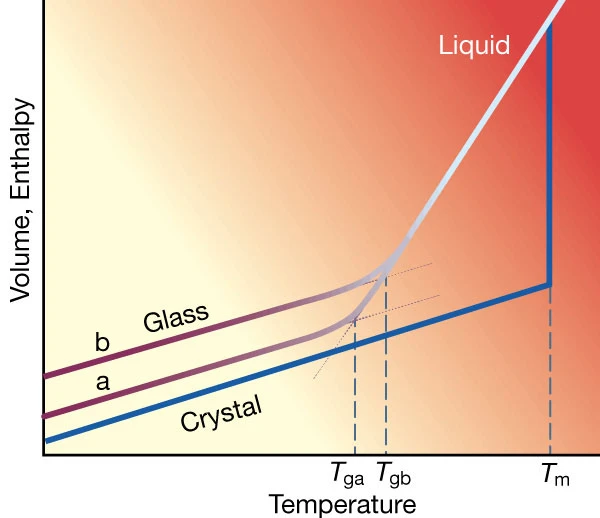
\includegraphics[width=12cm]{figs/fig_glassFormation.png}
	\centering
	\caption[{\em Schematic representation of cooling a liquid to lower temperatures}]{{\em Schematic representation of cooling a liquid to lower temperatures.} Behaviour of specific volume or enthalpy as a liquid is cooled below melting temperature $T_m$. Slow/fast cooling leads to the formation of glasses at lower/higher temperatures. \cite{debenedetti2001supercooled}\label{fig_glassFormation}}
    \end{figure}

%How fast the cooling should be to avoid the process of crystallization?

%Quenching of high temperature liquids to sufficiently low temperatures

A large number of colloidal systems, for example, paint, ink, ice cream, mayonnaise, photonic material, etc., are used in our everyday life and industries. The phase behaviour of many of these colloidal systems mimics the atomic systems. Hence, this provides a pathway to explore the various complex properties of atomic systems. Using advanced experimental techniques, supercooled and glassy phases of colloids have been obtained \cite{hunter2012physics}. Such experiments have been able to verify many theoretical proposals related to glassy systems \cite{hima2015direct}. In most colloidal systems, number density or packing fraction is the control parameter that can be tuned to obtain a supercooled or glassy state. Number density $\rho$ is defined as the number of particles per unit volume and packing fraction $\phi$ is defined as the fraction of the space occupied by the particles.

%%%%%%%%%%%%%%%%%%%%%%%%%%%%%%%%%%%%%%%%%%%%%%
\section{Characteristics of supercooled liquid and glass}
There are a variety of observations that one can make when the temperature/density of a glass-forming liquid is decreased/increased. These signatures are almost universal across different glass-formers. In the section below, we discuss some of these general characteristics in detail.

{\bf \em Dramatic increase in viscosity or slow dynamics:} As the supercooled liquid approaches the glass transition point, the dynamics of the liquid become drastically slow because the timescale of molecular rearrangement shows a dramatic increase and after some point, its viscosity becomes so high that it almost behaves like solid. One experimental definition of glass transition is given in terms of viscosity $\eta$: glass transition density or temperature is the point where viscosity becomes of the order of $10^{13}$ poise. If the logarithm of viscosity of different glass-forming liquids is plotted as a function of inverse temperature scaled by their respective glass transition temperatures (popularly known as Angell plot \cite{angell1995formation}), there is a clear difference in the functional dependence of different glass-formers: some of them, known as strong glass-formers, have Arrhenius type temperature dependence ($\eta \approx {\rm exp}(\Delta E/(k_BT))$, with $\Delta E$ as the effective activation energy of the liquid and $k_B$ as the Boltzmann constant) and others, known as fragile glass-formers, having significant deviation from Arrhenius behaviour (super-Arrhenius i.e., effective activation energy is more than that of Arrhenius case). In Fig.~\ref{fig_angell}, one such Angell plot shows examples of strong (with a straight line) and fragile glass-formers.
    
    \begin{figure}[hbt!]
	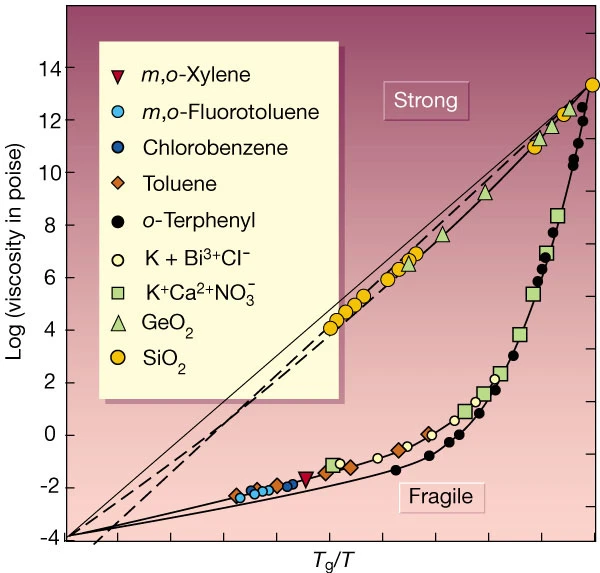
\includegraphics[width=12cm]{figs/fig_angell.png}
	\centering
	\caption[{\em Angell plot}]{{\em Angell plot.} The dependence of viscosity on inverse temperature scaled by the glass transition temperature $T_g$ for different glass-forming liquids.\cite{debenedetti2001supercooled}\label{fig_angell}}
    \end{figure}
    
The viscosity dependence on temperature of a wide class of glass-formers can be fitted with a phenomenological form, called Vogel-Fulcher-Tamann (VFT) form given by,

    \begin{equation}
        \eta(T) = \eta_{0}{\rm exp}(\frac{B}{T-T_{\rm VFT}}),
    \end{equation}
    
where $T_{\rm VFT}$ is the temperature at which viscosity is expected to diverge, meaning that this temperature should be very close to the glass transition temperature \cite{fulcher1992analysis,tammann1926abhangigkeit}.

A theoretical approach based on first principles, called {\em Mode Coupling Theory} (MCT) \cite{bengtzelius1984dynamics,reichman2005mode}, provides a sufficiently accurate description of relaxation dynamics of supercooled liquids in a certain regime of temperature or density. This theory predicts a critical temperature $T_{\rm MCT}$ or critical density $\rho_{\rm MCT}$, for the divergence of relaxation time or viscosity, which is found to be different from the experimentally observed glass transition temperature/density (also from the VFT temperature/density); typically MCT predicts a higher temperature or a lower density. The viscosity near the predicted mode coupling criticality has the power law divergence given by the form,

    \begin{equation}
        \eta(T) \sim (T-T_{\rm MCT})^{-\gamma},
    \end{equation}
    
with $\gamma$ as the exponent.

%%%%%%%%%%%%%%%%%%%%%%%%%%%%%%%%%%%%%%%%%%%%%%
    \subsection{Static structure}\label{structure}
    The difference between the structure of a liquid and a crystal is clearly identified: liquid is disordered and crystal has an order or arrangement in its constituents. Now, the question is, how does the structure of a liquid change when it is cooled to form supercooled liquid and further cooled to form glass? The simple answer is, the structure of liquid doesn't change much when cooled to form supercooled liquid or glass, meaning the structure of supercooled liquid and glass is also disordered. The most common way to look at the structure is using two-point density correlation function in real space (pair correlation function) and Fourier space (structure factor), as discussed below. Also, by calculating the local bond orientational order, the extent of possible crystalline order in the liquid can be estimated. Here, we discuss these quantities in detail which helps us to understand the structure of liquids.
    
    %%%%%%%%%%%%%%%%%%%%%%%%%%%%%%%%%%%%%%%%%%%%%%
    {\bf \em Pair correlation function:} The Pair correlation function $g(r)$ is defined in terms of particle positions ${\bf r}_i$ ($r$ is the inter-particle separation) for $N$ particle system with volume $V$,
    
    \begin{equation}
        g(r)=\frac{V}{N^2} \langle \sum_{i=1}^N \sum_{j=1,j\neq i}^N \delta(r-|\textbf{r}_j-\textbf{r}_i|)\rangle.
    \end{equation}
    
    \begin{figure}[hbt!]
	    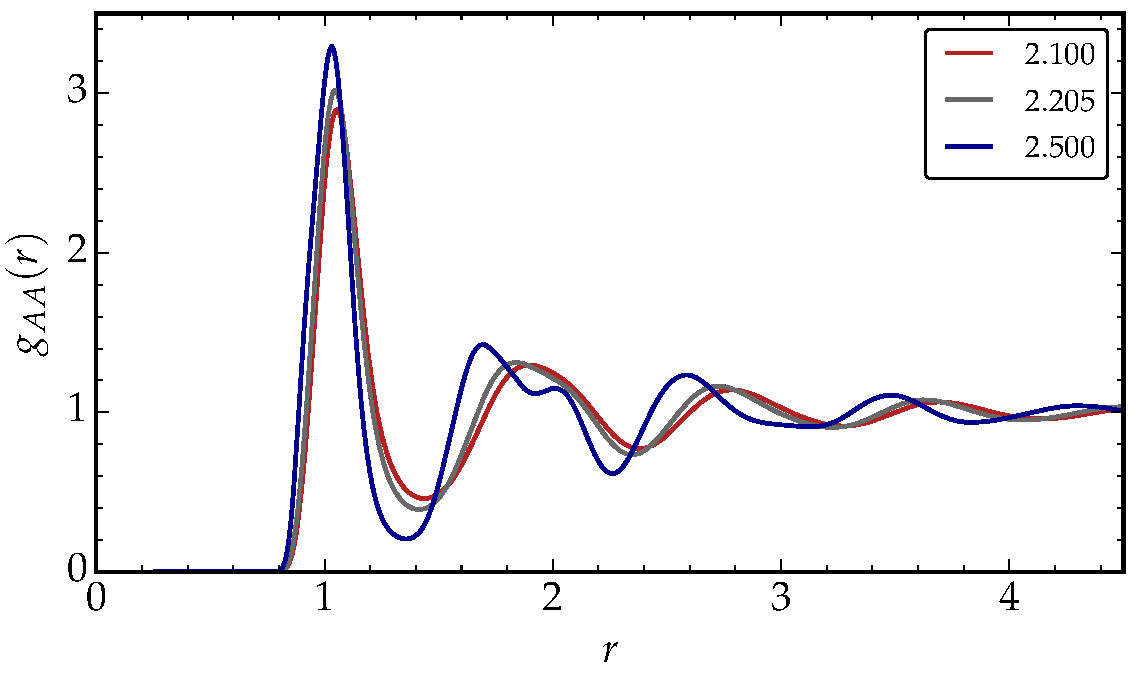
\includegraphics[width=14cm]{figs/fig_rdfAA.pdf}
	    \centering
	    \caption[{\em Pair correlation function}]{Pair correlation function calculated for bigger A-type particles using the glass-forming model in \cite{vaibhav2022finite}, at three different densities belonging to liquid state, supercooled liquid state and glassy state.\label{fig_rdf}}
    \end{figure}
    
    This function measures the probability of finding another particle at a distance $r$ from a particle, normalized by the uniform probability \cite{hansen2013,binder2011glassy}. If the pair correlation function is measured for an ideal gas then it will measure at all distances a value equal to $1$, because as per the definition of ideal gas, there is always a probability of finding the particle everywhere. For crystals, the particles are arranged in a periodic fashion, so pair correlation measurement shows sharp peaks. Although liquids have disordered arrangements of atoms, measurement of pair correlation shows a generic pattern. Measurement for short $r$ is zero due to the exclusion of particles in the intermediate surrounding of a particle, as particles have finite sizes. Then we have many oscillatory peaks and troughs beyond a finite value of $r$. Peaks signify the specific arrangement of particles in different shells as going radially away from a particle. Troughs after each peak are because of the exclusion of particles due to the particles in the previous shell. The pair correlation for a glass-forming liquid is shown in Fig.~\ref{fig_rdf}. It can be seen from here that the correlations become weaker with the increase in distance and for long distance there is almost no correlation, $g(r)$ becomes $1$ for large $r$.
    
%%%%%%%%%%%%%%%%%%%%%%%%%%%%%%%%%%%%%%%%%%%%%%
    {\bf \em Structure factor:} The local number density field in reciprocal space can be defined as follows \cite{hansen2013}:

    \begin{equation}
        \rho (\vec{q}) = \sum_{j=1}^{N} \exp \left( i \vec{q} \cdot {\vec{r}_j} \right)
        \label{eq_rhoqT}
    \end{equation}

    with $\vec{q}$ the wavevector and {$\vec{r}_j$} the position of the $j$'th particle. The autocorrelation function of the density variable, as defined by Eq.~(\ref{eq_rhoqT}), is the structure factor \cite{hansen2013,binder2011glassy},
    
    \begin{equation}
        S(\vec{q}) = \frac{1}{N} \langle \rho (\vec{q}) \rho (-\vec{q}) \rangle.
    \end{equation}
    
    Here, angular brackets represent ensemble average and $N$ is the total number of particles for which the calculation is done. The structure factor can be directly measured in scattering experiments. A typical calculation of structure factor for a glass-forming liquid looks very similar to as shown in Fig.~\ref{fig_sq}. Pair correlation and structure factor can also be related to each other using Fourier transform. So, in principle, the structure factor can be calculated from pair correlation but this leads to a loss of information, especially near the small $q$ values. Hence, it is advised to calculate $s(q)$ directly from the coordinates.
    
    \begin{figure}[hbt!]
	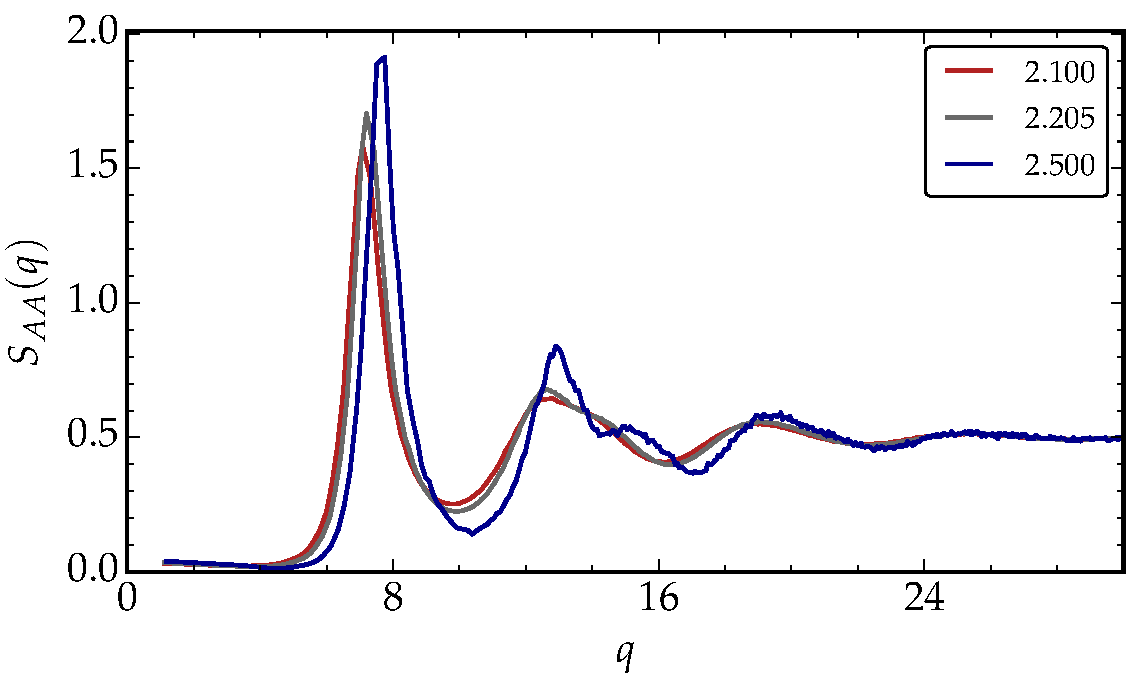
\includegraphics[width=14cm]{figs/fig_sq.pdf}
	\centering
	\caption[{\em Structure factor}]{Structure factor calculated for bigger A-type particles using the glass-forming model in \cite{vaibhav2022finite}, at three different densities belonging to liquid state, supercooled liquid state and glassy state.\label{fig_sq}}
    \end{figure}
    
    One thing that we can notice from the calculation of $g(r)$ and $s(q)$ in the above plots is that these calculations are not very sensitive in the vicinity of glass transition. Although, such calculations have been very useful in studying liquid to crystal transition. That is why, there are attempts to calculate higher order correlations beyond the two-point density-density correlations like $g(r)$ or $s(q)$ \cite{coslovich2013static,karmakar2014growing,luo2022many}. 
    %One such higher order four point density-density correlation function is $\chi_4$, which has been used in various studies to unravel hidden structural correlations.
    
    %%%%%%%%%%%%%%%%%%%%%%%%%%%%%%%%%%%%%%%%%%%%%%
    {\bf \em Pair correlation and structure factor for a binary mixture:} Since, we have simulated binary mixtures as model glass-formers, hence we also define different quantities for a binary mixture. For an AB mixture that contains a total number of $N = N_{\rm A} + N_{\rm B}$ particles.  
    
    The pair correlation function for the mixture can be defined as,
    \begin{equation}
        g_{\alpha\beta}(r)=\frac{V}{N_{\alpha}N_{\beta}} \langle \sum_{i=1}^{N_{\alpha}} \sum_{j=1}^{N_{\beta}} \delta(r-|\textbf{r}_j-\textbf{r}_i|)\rangle
    \end{equation}
    where $\alpha,\beta \in \{A,B\}$ and $\langle . \rangle$ indicates an ensemble average.
    
    The local number density in reciprocal space for particles of type $\alpha$ can be defined as follows \cite{hansen2013}:

    %
    \begin{equation}
    \rho_{\alpha} (\vec{q}) = \sum_{j=1}^{N_{\alpha}} \exp \left( i \vec{q} \cdot {\vec{r}_j^{\; (\alpha)}} \right)
    \label{eq_rhoq}
    \end{equation}
    %
    with $\vec{q}$ the wavevector and {$\vec{r}_j^{\; (\alpha)}$} the position of the $j$'th particle of type $\alpha$. The autocorrelation functions of the density variables, as defined by Eq.~(\ref{eq_rhoq}), are the partial structure factors \cite{hansen2013},
    
    
    %
    \begin{eqnarray}
    S_{\alpha \beta}(q) & = & \frac{1}{N} \left\langle \rho_{\alpha}(\vec{q}) \rho_{\beta}(- \vec{q}) \right\rangle \nonumber \\  
    & = & {\frac{1}{N}  \sum_{j=1}^{N_\alpha}  \sum_{k=1}^{N_\beta} \left\langle \exp\left[ - i \vec{q} \cdot \left( \vec{r}_j^{\; (\alpha)} - \vec{r}_k^{\; (\beta)} \right) \right] \right\rangle},
    \label{eq_spart}
    \end{eqnarray}
    %
    where $\langle . \rangle$ indicates an ensemble average.
    
    %%%%%%%%%%%%%%%%%%%%%%%%%%%%%%%%%%%%%%%%%%%%%%
    {\bf \em Concentration-concentration structure factor:} The concentration of A and B particles in binary mixture (as defined above) is given by $x_{\rm A} = N_{\rm A}/N$ and $x_{\rm B} = N_{\rm B}/N$, respectively. Also, from the densities (\ref{eq_rhoq}), we can introduce local concentration fluctuation variables \cite{hansen2013,interdiff} as
    %
    \begin{equation}
    c_\alpha (\vec{q}) = \rho_\alpha(\vec{q}) - x_\alpha \left( \rho_{\rm A}(\vec{q}) + \rho_{\rm B}(\vec{q}) \right) \, ,
    \end{equation}
    %
    describing the local deviation from a homogeneous distribution of particles of type $\alpha$. Since {$c_{\rm A} + c_{\rm B} = 1$}, the concentration variables are not independent of each other and it suffices to define {\it one} concentration-concentration structure factor for the binary mixture as
    %
    \begin{equation}
    S_{cc}(q) = \frac{1}{N} \left\langle c_{\rm A}(\vec{q}) c_{\rm A}(-\vec{q}) \right\rangle \, .
    \end{equation}
    %
    This function can be also expressed as a linear combination of the partial structure factors,
    %
    \begin{equation}
    S_{cc}(q) = x_B^2S_{\rm AA}(q)+x_{\rm A}^2 S_{\rm BB}(q) - 2x_{\rm A} x_{\rm B} S_{\rm AB}(q).   
    \end{equation}
    %
    In the limit $q\to \infty$, $S_{cc}(q)$ approaches $x_{\rm A} x_{\rm B}$, corresponding to the concentration-concentration structure factor of an ideal binary mixture. In the limit $q\to 0$, $S_{cc}(q)$ is related to the concentration susceptibility and thus to the second derivative of the Gibbs free energy $G$ with respect to $x_{\rm A}$ and $x_{\rm B}$ via
    %
    \begin{equation}
    \Phi = \frac{x_{\rm A} x_{\rm B}}{k_{\rm B} T} \frac{\partial^2 G}{\partial x_{\rm A} x_{\rm B}} = \frac{x_{\rm A} x_{\rm B}}{S_{cc}(q=0)} \, ,
    \label{eq_phi}
    \end{equation}
    %
    with $k_{\rm B}$ the Boltzmann constant. In chapter-\ref{chap6}, we use Eq.~(\ref{eq_phi}) to compute the thermodynamic factor from an extrapolation of $S_{cc}(q)$ to $q=0$.
    
    %%%%%%%%%%%%%%%%%%%%%%%%%%%%%%%%%%%%%%%%%%%%%%
    {\bf \em Bond orientational order parameter:} Sometimes, it is important to check the local structure of the liquid to ensure any developing local crystalline order. Such analysis can be done by calculating the local bond order parameters that have been proposed by Steinhardt {\it et al.}~\cite{steinhardt1983}. At first, we need to identify the nearest neighbours for each particle within a cutoff ($N_b(i)$ is the number of such neighbours for each particle $i$). After this, for each particle, a complex local orientational order vector $q_{lm}(i)$ with $(2l+1)$ components is constructed using the following definition:

    %
    \begin{equation}
    \label{qlm}
    q_{lm}(i) =\frac{1}{N_b(i)} \sum_{j=1}^{N_b(i)} Y_{lm}(\hat{r}_{ij}).
    \end{equation}
    %
    
    Here, $Y_{lm}(\hat{r}_{ij})$ is the spherical harmonic of degree $l$ and order $m$. As per definition, $l$ is always a non-negative integer and $m$ can take the integral values from $m = -l$ to $m = l$ for a given value of $l$. $\vec{r}_{ij}$ is the vector from the particle $i$ to particle $j$ and $\hat{r}_{ij}$ is the corresponding unit vector. Now, as suggested in Ref.~\cite{dellago2008}, the locally averaged quantity $\bar{q}_{lm}(i)$ is calculated for each particle $i$, using

    %
    \begin{equation}
    \bar{q}_{lm}(i) = \frac{1}{\tilde{N}_b(i)} \sum_{k=0}^{\tilde{N}_b(i)} q_{lm}(k),
    \end{equation}
    %
    
    where averaging (summation from $k=0$ to $\tilde{N}_b(i)$) has been done over the neighboring particles of $i$ (as above defined, based on the cutoff) and particle $i$ itself. Such averaging procedure takes into account even the information of the structure beyond the cutoff and has shown better identification of crystal structures in simulations. Using these averaged forms of local bond order vector components a norm $\bar{q}_{l}(i)$ is defined for each particle:

    %
    \begin{equation}
    \bar{q}_{l}(i) = \sqrt{\frac{4\pi}{2l+1} \sum_{m=-l}^{l} |\bar{q}_{lm}(i)|^2}.
    \end{equation}
    %
    
    Depending on the definition of the spherical harmonics used, the factor $\frac{4\pi}{2l+1}$ before summation in the above equation, is used or not used. This quantity $\bar{q}_{l}(i)$ is sensitive to different crystal structure systems depending on the choice of $l$. Especially, bond orientational order parameter for $l = 4$ and $l = 6$ have been used to identify structures similar to cubic and hexagonal systems. We have done this analysis of bond orientational order parameter in chapter-\ref{chap6} to detect the presence of crystalline nuclei in a binary liquid mixture
    
%%%%%%%%%%%%%%%%%%%%%%%%%%%%%%%%%%%%%%%%%%%%%%%
    \subsection{Dynamics}\label{dynamics}
    
    The dynamics of a glassy liquid can be characterized at a single particle level using {\em Mean Squared Displacement} and also the time evolution of structural correlations can be quantified using quantities like {\em Intermediate scattering function}. Here, we discuss these quantities one by one.
    
    {\bf \em Mean squared displacement:} This can be calculated by tracking the trajectory of each particle, which can be defined as,
    
    \begin{equation}
        \langle \delta \textbf{r}^2(t)\rangle = \frac{1}{N}  \sum_{j=1}^{N} \left\langle \left(\textbf{r}_j(t) - \textbf{r}_j(0) \right)^2 \right\rangle.
    \end{equation}
    
    Here, $\textbf{r}_j(t)$ is the position of particle $j$ at time $t$, $N$ is the number of particles and the angular brackets represent ensemble average over different initial conditions.
    
    \begin{figure}[hbt!]
	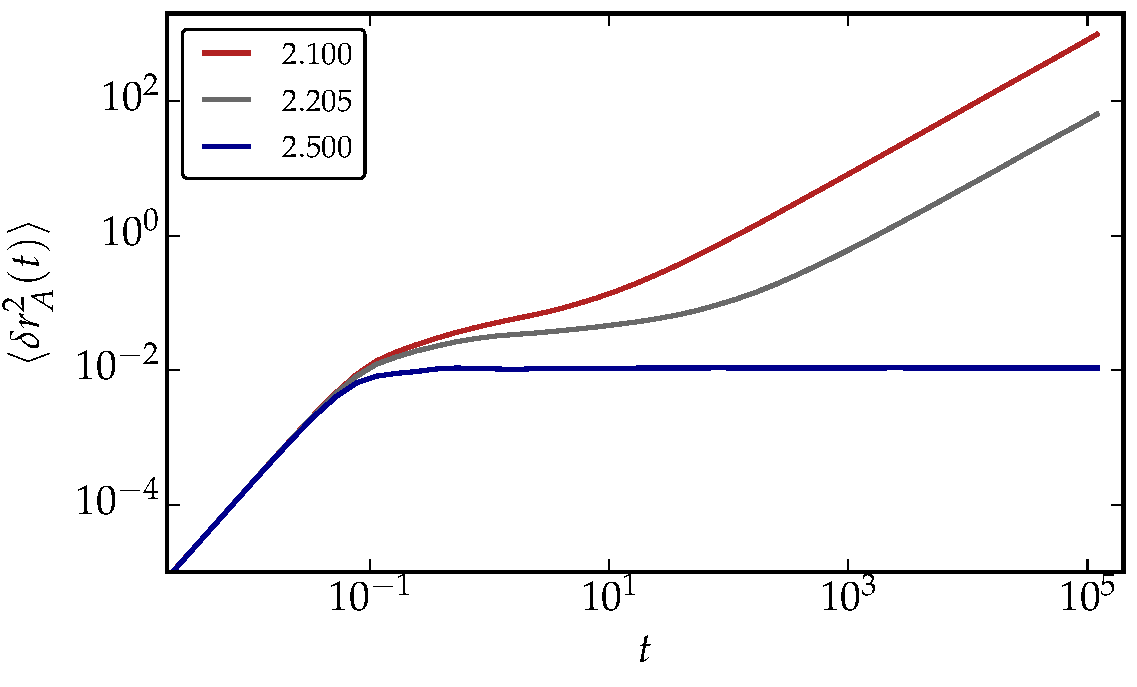
\includegraphics[width=14cm]{figs/fig_msd.pdf}
	\centering
	\caption[{\em Mean squared displacement}]{Mean squared displacement calculated for bigger A-type particles using the glass-forming model in \cite{vaibhav2022finite}, at three different densities belonging to liquid state, supercooled liquid state, and glassy state.\label{fig_msd}}
    \end{figure}
    
    Fig.~\ref{fig_msd} shows the measurements for a glass-forming liquid at three different densities.  At very short times, the behaviour of mean squared displacement is proportional to $t^2$, which corresponds to free-particle (or 'ballistic') motion \cite{hansen2013,frenkel2001understanding}. This is identical to the motion of ideal gas. The long time behaviour of mean squared displacement at density $2.100$ and $2.205$ is proportional to $t$ which can also be related to diffusion coefficient as discussed below \ref{selfInter}. But at density $2.500$, the long time diffusion is not visible. Rather, the plateau after the ballistic regime extends over a large time window, as the density increases. This is indicating the average time scale at which the cage breaking is happening is increasing with time and eventually becomes extremely delayed, which is a signature of slower glassy dynamics with the increase in density.

    %%%%%%%%%%%%%%%%%%%%%%%%%%%%%%%%%%%%%%%%%%%%%%
  %  {\bf \em Time correlation functions:} Let's consider two dynamical variables $A(t)$ and $B(t)$ then the time correlation function of these two variables is defined as,
    
  %  \begin{equation}
   %     C_{AB}(t,t')= \langle A(t+t') B^*(t') \rangle
  %  \end{equation}
    
   % where $B^*(t)$ is the complex conjugate of $B(t)$. For equilibrium system (or sometimes for nonequilibrium systems in steady state), the correlation function is independent of the time origin i.e., independent of $t'$. Calculation of such correlations can be useful in identifying any temporal pattern present in the system. Also, the time integrals of time correlation functions can be related with macroscopic transport coefficients via Green-Kubo relations \cite{mcquarrie1973statistical} \cite{hansen2013}.

    %%%%%%%%%%%%%%%%%%%%%%%%%%%%%%%%%%%%%%%%%%%%%%
    {\bf \em Incoherent intermediate scattering function:} At a single-particle level, we consider the incoherent intermediate scattering function $F_{\rm s}^{\alpha}(q,t)$ of a tagged particle of type $\alpha$. This is the correlation function of the time-displaced one-particle density and is defined by \cite{hansen2013}
    %
    \begin{equation}
    F_{\rm s}^{\alpha}(q,t) = \frac{1}{N_{\alpha}}  \sum_{j=1}^{N_\alpha} \left\langle \exp \left[ -i \vec{q}\cdot {\delta \vec{r}_j^{\; (\alpha)}(t)} \right] \right\rangle \, ,
    \end{equation}
    %
    
    \begin{figure}[hbt!]
	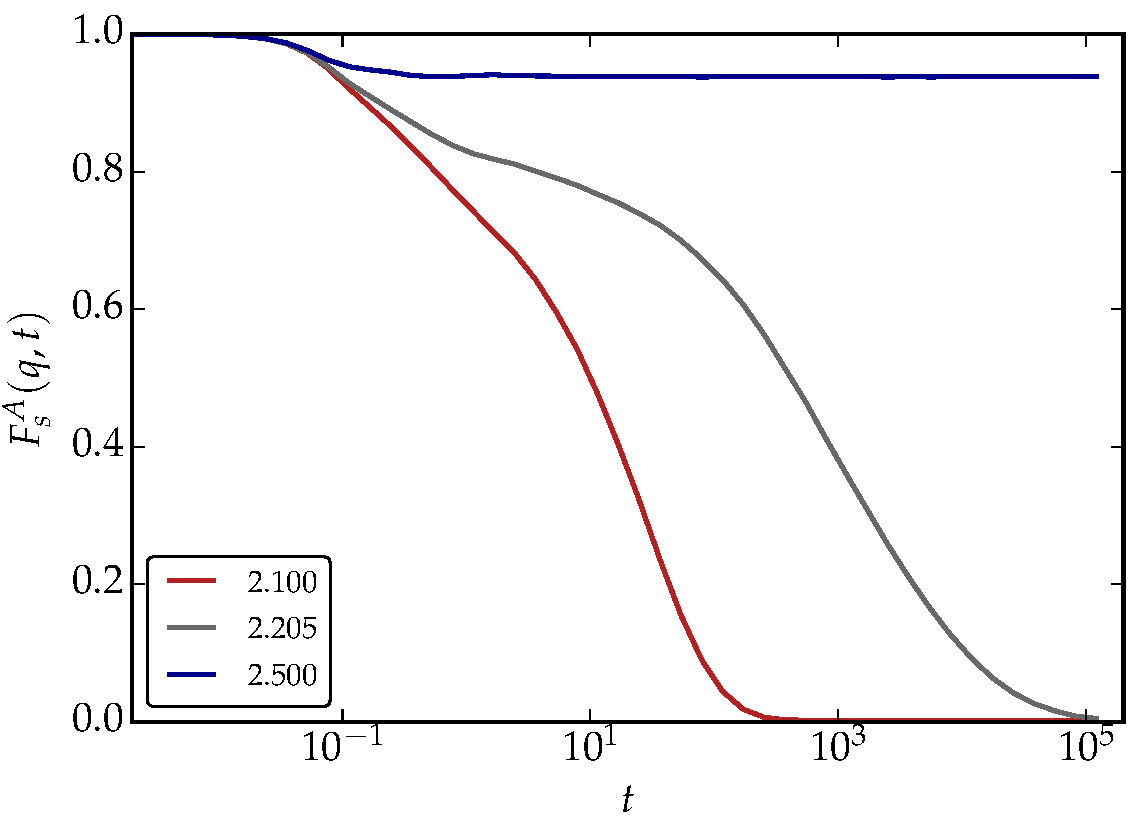
\includegraphics[width=14cm]{figs/fig_fsqt.pdf}
	\centering
	\caption[{\em Self intermediate scattering function}]{Self intermediate scattering function calculated for bigger A-type particles using the glass-forming model in \cite{vaibhav2022finite}, at three different densities belonging to liquid state, supercooled liquid state, and glassy state.\label{fig_fsqt}}
    \end{figure} 
    
    where $\delta \vec{r}_j^{\; (\alpha)}(t)= \vec{r}_j^{\; (\alpha)}(t) - \vec{r}_j^{\; (\alpha)}(0)$ describes the displacement of particle $j$ of type $\alpha$ from its position $\vec{r}_j^{\; (\alpha)}(0)$ at time 0 to the position $\vec{r}_j^{\; (\alpha)}(t)$ at time $t$. Of special interest for the analysis of the dynamics of glass-forming liquids is the decay of $F_{\rm s}^{\alpha}(q,t)$ as a function of time around values of $q$ corresponding to the location of the first peak of the static structure factor, $q_{\rm max}$. This is due to the fact that the slowing down of structural relaxation of the glass-forming liquid is associated with the cage effect \cite{binder2011} and the typical size of a cage is of the order of $2 \pi/q_{\rm max}$. The measurement of the incoherent intermediate scattering function for the glassy mixture has been plotted in Fig.~\ref{fig_fsqt}, where we can see the two-step relaxation process.
    
    %%%%%%%%%%%%%%%%%%%%%%%%%%%%%%%%%%%%%%%%%%%%%%
    {\bf \em van Hove correlation function:} The self part of van Hove correlation function $G_s(x,t)$ is defined as \cite{hansen2013}:
    
    \begin{equation}
        G_s(x,t) =\frac{1}{N} \sum_{i=1}^N \delta(x-(x_i(t)-x_i(0))).
    \end{equation}
    
    \begin{figure}[hbt!]
    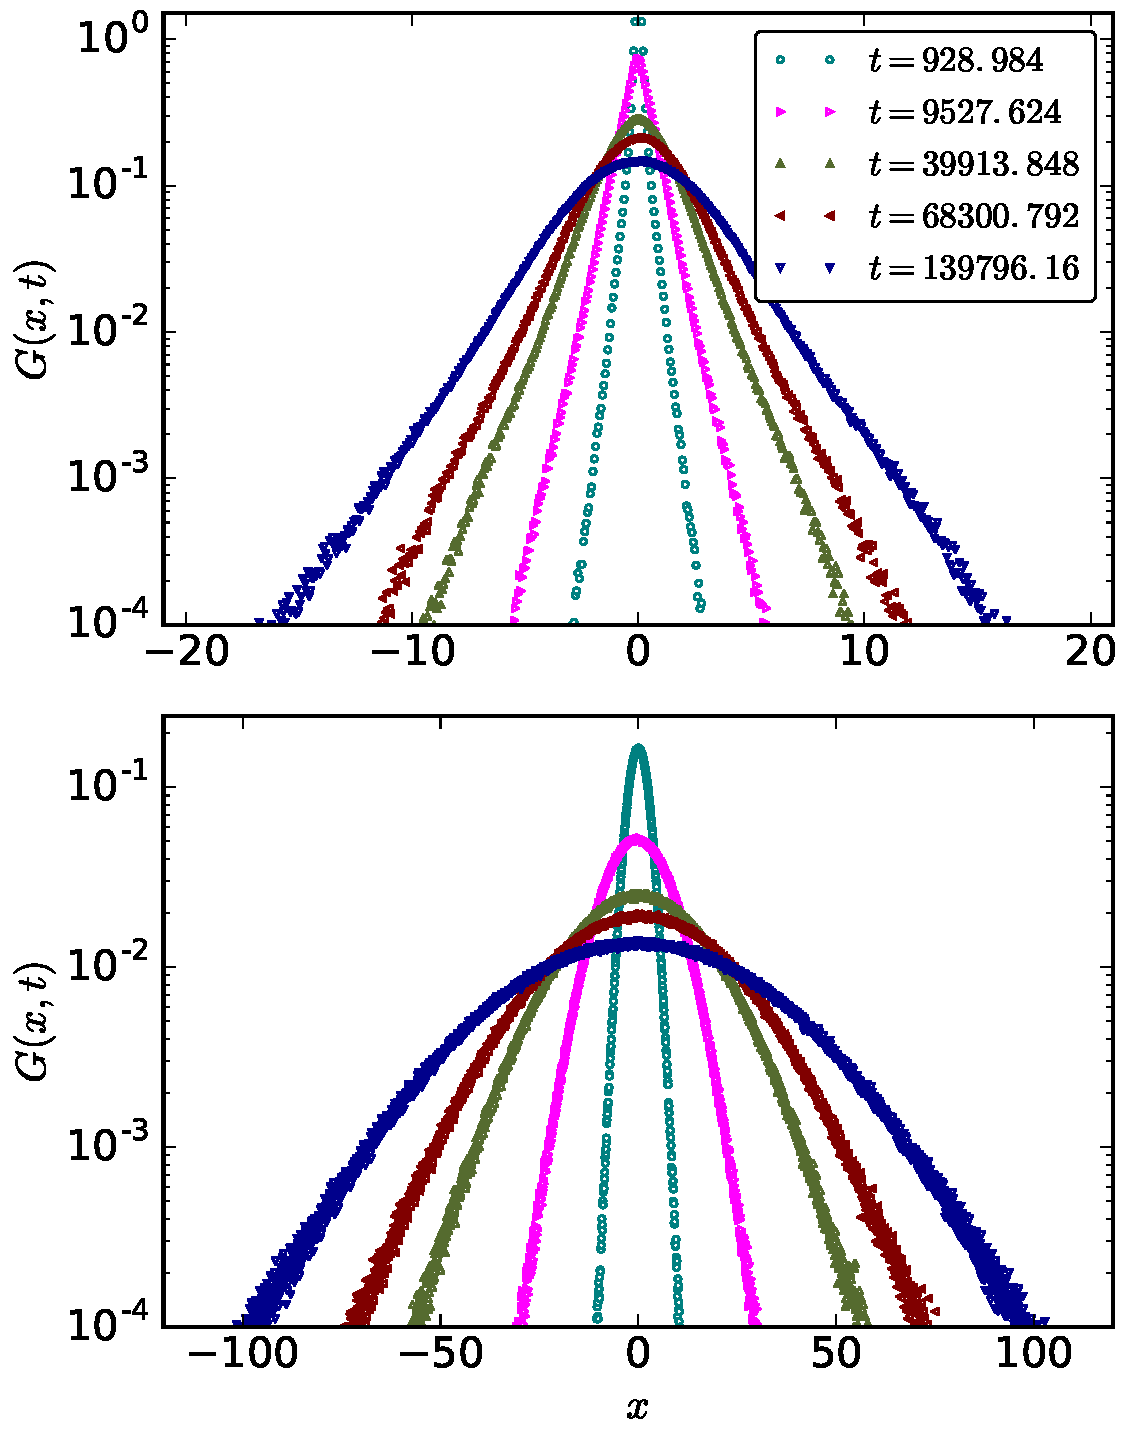
\includegraphics[width=12cm]{figs/fig_vanHove.pdf}
    \centering
    \caption[\em van Hove correlation function]{The van Hove correlation function at different times (marked) at temperature $T=0.45$ in upper panel and $T=0.7$ in lower panel for Kob-Andersen binary Lennard-Jones glass-forming mixture \cite{kob1995testing}.\label{fig_vanHove}}
    \end{figure}

    The normalized correlation function actually measures the probability of a particle having displacement $x$ in time $t$. This is an important measurement to characterize the fluctuation in the distribution of particle displacements. For high temperature liquids, this function quickly reaches a Gaussian form. But, for supercooled liquids and glasses, the behaviour shows a strong deviation from Gaussianity, as shown in Fig.~\ref{fig_vanHove} for a glass-forming liquid at two different temperatures and different times. In the supercooled states, the Gaussian shape is recovered at very long times characterized by the typical structural relaxation time at any temperature. We have used this observable in Chapter-\ref{chap6} to understand the impact of shear on particle displacements. 
    
%%%%%%%%%%%%%%%%%%%%%%%%%%%%%%%%%%%%%%%%%%%%%%%
    \subsection{Selfdiffusion and interdiffusion}\label{selfInter}
    
    For a liquid mixture, as defined above, the single particle dynamics is studied using MSD (also discussed in \ref{dynamics} ), which can be measured for the different types of species present in the system to calculate their respective selfdiffusion coefficients. This gives the idea of the dynamical  behaviour of different species in the mixture. But, to understand the intermixing properties of different species present in the system,  we calculate interdiffusion properties by monitoring the dynamics of center of mass of each species type \cite{interdiff}. Hence, interdiffusion is related to the relaxation of concentration of different species in the mixture. Here, we discuss the phenomena of selfdiffusion and interdiffusion in detail.

    %%%%%%%%%%%%%%%%%%%%%%%%%%%%%%%%%%%%%%%%%%%%%%
    {\bf \em Selfdiffusion:} For a liquid mixture, $\delta \vec{r}_j^{\; (\alpha)}(t)= \vec{r}_j^{\; (\alpha)}(t) - \vec{r}_j^{\; (\alpha)}(0)$ describes the displacement of particle $j$ of type $\alpha$ from its position $\vec{r}_j^{\; (\alpha)}(0)$ at time 0 to the position $\vec{r}_j^{\; (\alpha)}(t)$ at time $t$.
    
    We determine the selfdiffusion coefficient of a tagged particle of type $\alpha$ from the mean-squared displacement (MSD), defined by
    %
    \begin{equation}
    \label{eq_msd}
    { {\rm MSD}_\alpha (t) =  \frac{1}{N_{\alpha}}  \sum_{j=1}^{N_\alpha} \left\langle \left( \delta \vec{r}_j^{\; (\alpha)}(t) \right)^2 \right\rangle} \, .
    \end{equation}
    %
    The corresponding selfdiffusion coefficient $D_\alpha$ is obtained from the long-time limit of {${\rm MSD}_{\alpha}(t)$} via the Einstein relation \cite{hansen2013, binder2011}
    %
    \begin{equation}
    { D_{\alpha} = \lim_{t \to \infty} \frac{{\rm MSD}_{\alpha}(t)}{6t}.}
    \label{eq_ds}
    \end{equation}
    %
    
    %%%%%%%%%%%%%%%%%%%%%%%%%%
    {\bf \em Interdiffusion:} If $\vec{R}_{\rm A}(t)$ is defined as the center-of-mass coordinate of the A particles at time $t$,
    %
    \begin{equation}
    { \vec{R}_{\rm A}(t) = \frac{1}{N_{\rm A}} \sum_{j=1}^{N_{\rm A}} \vec{r}_j^{\rm \; (A)}(t)} \, .
    \end{equation}
    %

    The interdiffusion coefficient $D_{\rm AB}$ can be also calculated from an Einstein relation, i.e.~from the long-time limit of a MSD. In this case, the MSD of the variable $\vec{R}_{\rm A}(t)$ has to be considered,

    %
    \begin{eqnarray}
    {\rm MSD}_{\rm cmA} 
    & = & \left\langle \left[ \vec{R}_{\rm A}(t) - \vec{R}_{\rm A}(0) \right]^2 \right\rangle \nonumber \\
    & = & \frac{1}{N_{\rm A}^2} \left\langle \sum_{k = 1}^{N_{\rm A}} \sum_{l = 1}^{N_{\rm A}} \delta \vec{r}_k^{\rm \; (A)}(t) \delta \vec{r}_l^{\rm \; (A)}(t) \right\rangle 
    \label{eq_msdcm}
    \end{eqnarray}
    %

    Then, the interdiffusion coefficient is given by \cite{horbach2007}
    %
    \begin{equation}
    D_{\rm AB} = \Phi L \, ,
    \label{eq_dab}
    \end{equation}
    %
    where $\Phi$ is the thermodynamic factor, as defined by Eq.~(\ref{eq_phi}), and the Onsager coefficient
    %
    \begin{equation}
    { L = \left[ 1+ \frac{x_{\rm A}}{x_{\rm B}} \right]^2 N x_{\rm A} x_{\rm B} \lim_{t\to \infty} \frac{{\rm MSD}_{\rm cmA}(t)}{6t}} \, ,
    \label{eq_onsager}
    \end{equation}
    %
    describes the kinetic part of $D_{\rm AB}$. 

    Using
    %
    \begin{equation}
    \sum_{j=1}^{N_{\rm A}} \delta \vec{r}_j^{\rm \; (A)}(t) = 
    - \sum_{j=1}^{N_{\rm B}} \delta \vec{r}_j^{\rm \; (B)}(t) \, ,
    \end{equation}
    %
    it is easy to show that Eq.~(\ref{eq_onsager}) for the Onsager coefficient $L$ is equivalent to the following equation:
    %
    \begin{equation}
    L = \lim_{t\to \infty} \frac{1}{6t} \left[ x_{\rm A} {\rm MSD}_{\rm B}(t)
    + x_{\rm B} {\rm MSD}_{\rm A}(t) + x_{\rm A} x_{\rm B} {\rm MSD}_{\rm cross}  \right] \, ,
    \label{eq_onsager2}
    \end{equation}
    %
    where ${\rm MSD}_{\rm cross}$ quantifies the cross correlations of particle displacements,
    %
    \begin{eqnarray}
    {\rm MSD}_{\rm cross} & = &
    \frac{1}{N x_{\rm A}^2} \left\langle \sum_{\substack{k,l \\ k\neq l}} \delta \vec{r}_k^{\rm \; (A)}(t) \delta \vec{r}_l^{\rm \; (A)}(t) \right\rangle \nonumber \\
    & & + \, \frac{1}{N x_{\rm B}^2} \left\langle \sum_{\substack{k,l \\ k\neq l}} \delta \vec{r}_k^{\rm \; (B)}(t) \delta \vec{r}_l^{\rm \; (B)}(t) \right\rangle \nonumber \\
    & & - \, 2 \frac{1}{N x_{\rm A} x_{\rm B}} \left\langle \sum_{k,l} \delta \vec{r}_k^{\rm \; (A)}(t) \delta \vec{r}_l^{\rm \; (B)}(t) \right\rangle \, .
    \label{eq_msdcross}
    \end{eqnarray}
    %
    With Eqs.~(\ref{eq_onsager2}) and (\ref{eq_msdcross}), the interdiffusion coefficient $D_{\rm AB}$ can be written as a linear combination of the selfdiffusion coefficients,
    %
    \begin{equation}
    D_{\rm AB} = \Phi S \left( x_{\rm A} D_{\rm B} + x_{\rm B} D_{\rm A} \right) \, ,
    \label{eq_dabdarken}
    \end{equation}
    %
    where the ``Manning factor'' \cite{manning1961} $S$ contains all the cross correlations \cite{horbach2007} that contribute to $L$ and is defined by
    %
    \begin{equation}
    S = 1 + \frac{1}{x_{\rm A} D_{\rm B} + x_{\rm B} D_{\rm A}} {\rm lim}_{t \to \infty} \frac{x_{\rm A} x_{\rm B} {\rm MSD}_{\rm cross}}{6t}    
    \end{equation}
    %
    The value $S = 1$ implies vanishing cross correlations \cite{akcasu1997, horbach2007}. In this case, the interdiffusion can be expressed as a linear combination of selfdiffusion coefficients, leading to Darken equation given by,
    
    %
    \begin{equation}
    D_{\rm AB} = \Phi \left( x_{\rm A} D_{\rm B} + x_{\rm A} D_{\rm A} \right).
    \end{equation}
    %

    %Connecting structure and dynamics (ML approach)
    %\subsection{Theoretical understanding:} Since, VFT form has no theoretical basis, Potential Energy Landscape picture, Mode Coupling Theory(MCT), Kinetically constrained model, Entropy theory of Adam, Gibbs and Di Marzio’s, Free volume theory of glasses, Random First Order Transition Theory
    

\section{Thermal response of glasses}
As discussed in the introductory section of this chapter, understanding the response of glassy materials to thermal gradient is important for various applications \cite{hufnagel2015cryogenic,schuh2007mechanical,koehler2016}. Transport of heat, mass, and charge are irreversible processes, governed by phenomenological laws, viz. Fourier's law, Fick's law, and Ohm's law. But, we have various occasions in real life where more than one such transport processes take place simultaneously. For example, consider the Peltier effect, where applying a voltage gradient causes charge flow and also the development of temperature gradient or heat flow. Here two irreversible transport processes, charge transport and heat transport are interfering with each other \cite{degroot}. We have many such examples of cross effects, as shown in the schematic in Fig.~\ref{schematicCross}. One such cross effect that becomes important when a temperature gradient is applied to liquid mixtures, is known {\em Soret effect}, as discussed below. We are interested in heat transport in liquid mixtures because most of the good glass-formers are mixtures and our aim is to study the response of glasses in the presence of a thermal gradient.
    
    \begin{figure}[hbt!]
	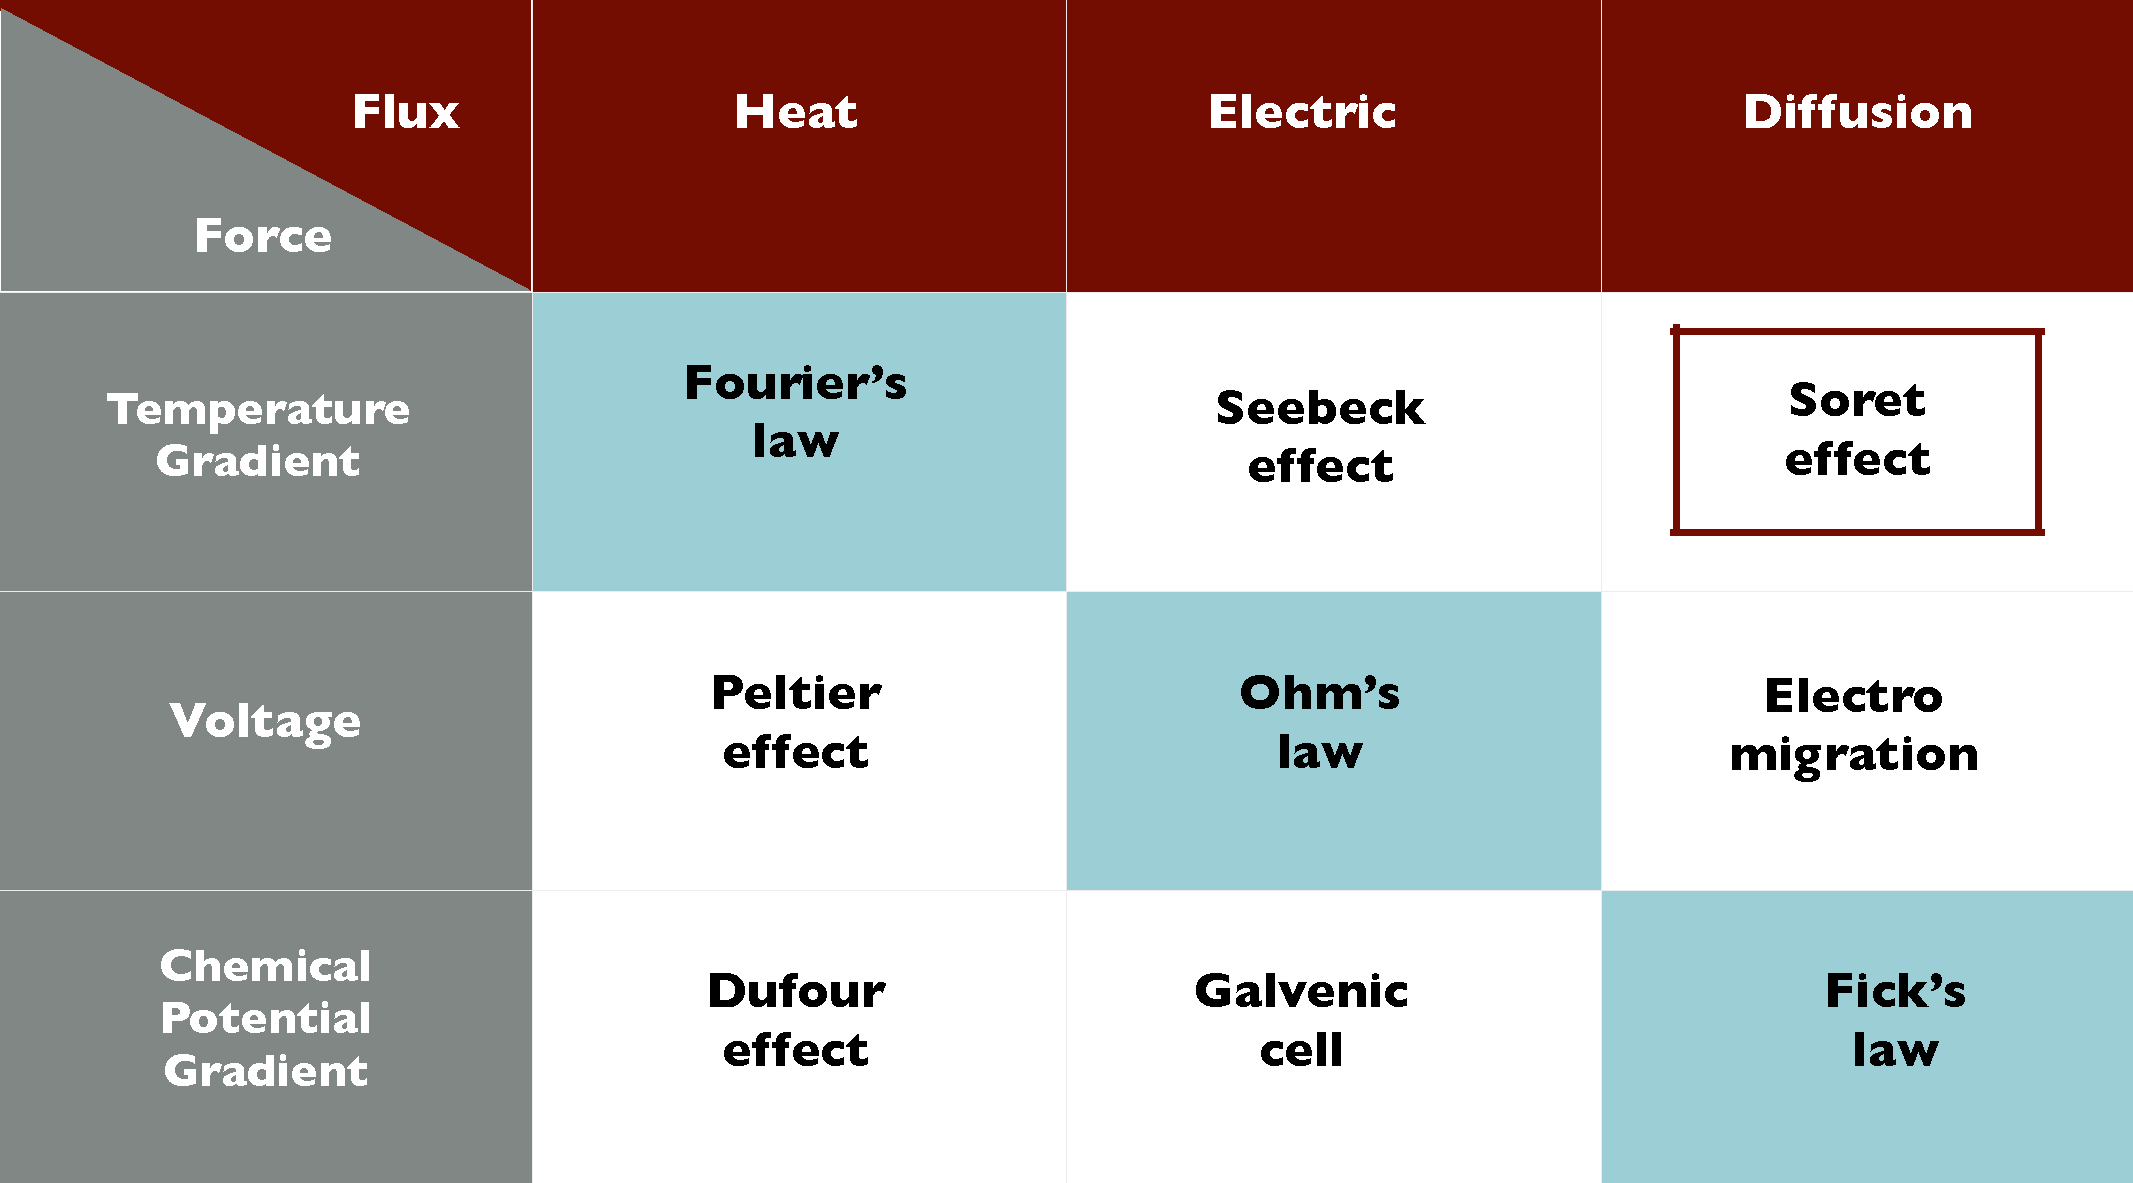
\includegraphics[width=14cm]{figs/schematicCross.pdf}
	\centering
	\caption[{\em Interferring irreversible transport processes}]{Different cross effects with either one irreversible transport process (along diagonal) or two such processes (off-diagonal). In the case of Soret effect, a temperature gradient is imposed resulting in heat and mass transport \cite{degroot}.\label{schematicCross}}
    \end{figure}
    
    \subsection{Heat transport in liquid mixtures: thermophoresis}
    
     \begin{figure}[hbt!]
	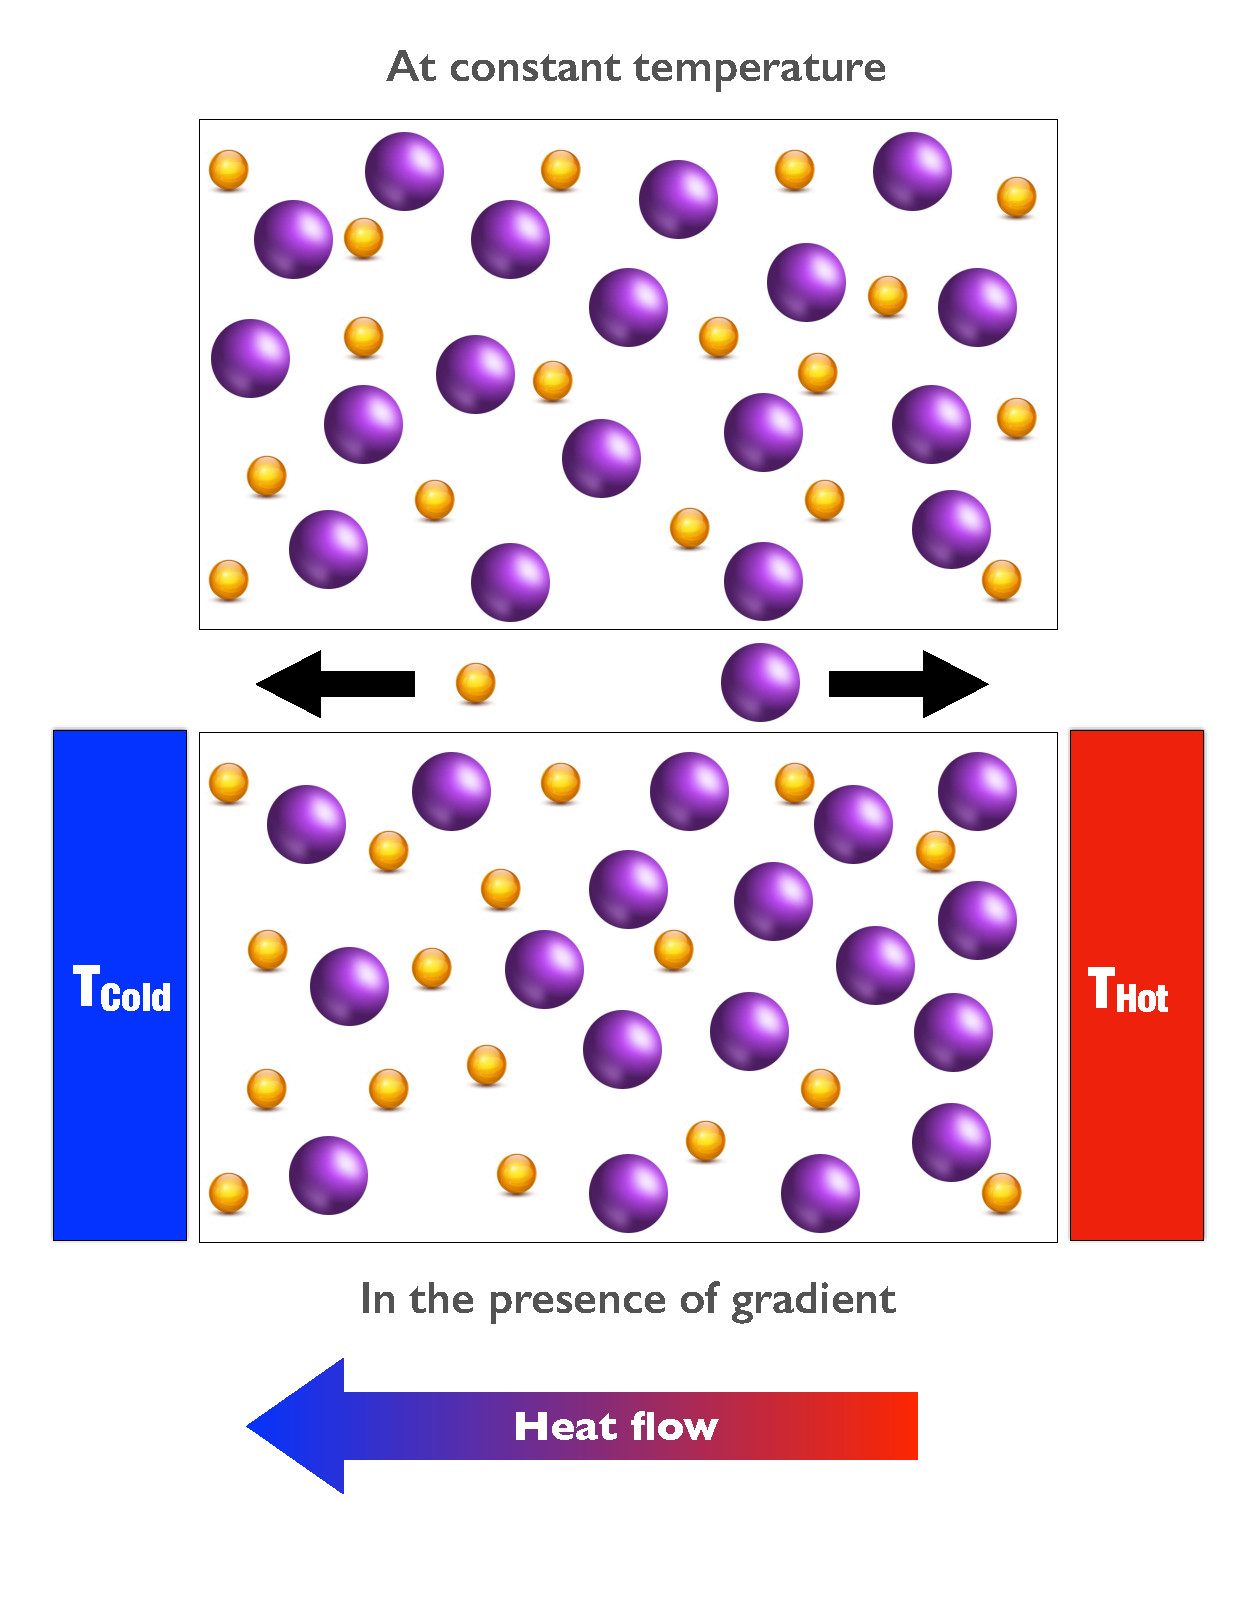
\includegraphics[width=14cm]{figs/thermophoresis.pdf}
	\centering
	\caption{{\em Schematic showing thermophoresis.}  \label{thermophoresis}}
    \end{figure}
    
    Now, we discuss the process of heat transport in Onsager's formalism of phenomenological theory of irreversible processes \cite{degroot}. In this formalism, total entropy production $\sigma$ happening in the system is written in terms of thermodynamic forces $X_i$ and fluxes $J_i$:
    \begin{equation}
        \sigma = \sum_i J_i X_i.
    \end{equation}
    
    For each transport process happening in the system, the corresponding flux can be written as a linear superposition of different thermodynamic forces,
    \begin{equation}
        J_i = \sum_k L_{ik}X_k.
    \end{equation}
    
    Here, $L_{ik}$ are called phenomenological coefficients. combining the above two equations,
    \begin{equation}
        \sigma = \sum_{i,k} L_{ik} X_i X_k.
    \end{equation}
    It can be shown that all phenomenological coefficients are not independent and the cross coefficients are symmetric (Onsager reciprocity relation): $L_{ij} = L_{ji}$.
    
    Let's consider the same binary liquid mixture with the concentration of one species $x_A$ and another species $x_B = 1-x_A$, as defined above, and write the heat and mass transport processes along with the entropy production in the presence of thermal gradient:
    \begin{equation}
        \sigma = -\frac{1}{T^2} J_q \nabla T - \frac{1}{T} J_A \mu_{AA} (x_A+x_B)/x_B \nabla x_A.
    \end{equation}
    
    Here, $T$ is the temperature, $J_q$ is the heat flux, $J_A$ is the mass flux of one kind of species in the mixture, and $\mu_{AA}$ is the chemical potential. The mass flux of the first species and second species are actually connected with each other due to the coupled motion. So, the flux of any of the species can be considered. Now the phenomenological equations can be written for $J_q$ and $J_A$,
    
    \begin{equation}
        J_q = -L_{qq} \frac{\nabla T}{T^2} - L_{qA} \frac{\mu_{AA}}{x_BT}\nabla x_A
    \end{equation}
    
    \begin{equation}
        J_1 = -L_{Aq}\frac{\nabla T}{T^2} - L_{AA} \frac{\mu_{AA}}{x_BT}\nabla x_A.
    \end{equation}
    
    If we define, $D_{AB} = L_{AA}\mu_{AA}/(\rho x_BT)$ as interdiffusion coefficient and $D_T = L_{Aq}/(\rho x_Ax_BT^2)$ as thermal diffusion coefficient then in the steady state when mass flux vanishes i.e., $J_A = 0$, the Soret coefficient ($S_T$) defined as the ratio of thermal diffusion coefficient to mass diffusion coefficient, can be written as:
    
    \begin{equation}
        S_T = \frac{D_T}{D_{AB}} = -\frac{1}{x_Ax_B} \frac{\nabla x_A}{\nabla T}.
    \end{equation}
    
    From the above discussion on the Soret effect, we see that when a liquid mixture is put under a constant temperature environment then the composition is spatially uniform but under the influence of an external temperature gradient, different particles respond differently, setting up a mass flux resulting into a nonuniform spatial composition. This is schematically shown in Fig.~\ref{thermophoresis}. We discuss this aspect in the context of a glassy liquid in Chapter-\ref{chap3}.
    
   

\section{Mechanical response of glasses}
In earlier sections, we discussed the importance of a fundamental understanding of the mechanical response of glasses. One way of studying the mechanical deformation is via shear i.e., applying a force parallel to the surface to cause the deformation \cite{chhabra2011non,larson}. Other ways could be via compression or stretching i.e., applying a deforming force (load) perpendicular to the surface \cite{chaudhuri2016structural}. Here, we are mainly interested in studying the shear response of glassy systems via a uni-directional deformation at a fixed rate, where a surface of the material is sheared in a direction with a fixed rate\footnote{Another very popular approach to shear the material is oscillatory shear protocol, where the material is sheared to and fro in a cyclic fashion.}. In general, the mechanical state of the material is characterized via the stress tensor for quantifying the extent of forcing that has developed or is being applied. Alternatively, one can use the strain tensor to characterize the degree of deformation. In typical experimental situations, e.g. in the case of uni-directional deformation discussed above, only one element of the tensor becomes finite. However, this can be generalized for more complex forcings where it can be a combination of different components of the tensor. 

In this section, we summarize different characteristics associated with the shear deformation of glassy systems.

    %%%%%%%%%%%%%%%%%%%%%%%%%%%%%%%%%%%%%%%%%%%%
    \subsection{Couette flow}
    
    Let's consider a liquid in a planar Couette flow geometry \cite{larson,chhabra2011non} (see Fig.~\ref{couetteFlow}) such that the $xy$-plane is deformed with fixed shear rate $\dot{\gamma}$ in $x$-direction. As mentioned above, this can be achieved in experiments by putting fluid between two plates and moving one of the plates or both plates with a fixed rate, but in simulations, one way of achieving this is via modifying the boundary conditions or equations of motion. For the given geometry in Fig.~\ref{couetteFlow} where flow is in the x-direction, flow velocity as a function of height $y$ is given by $v_x(y) = \dot{\gamma} y$. The $x$-direction is called the flow direction, $y$ is the gradient direction (because velocity spatially varies in this direction) and $z$ is known as vorticity direction.
    
    \begin{figure}[hbt!]
	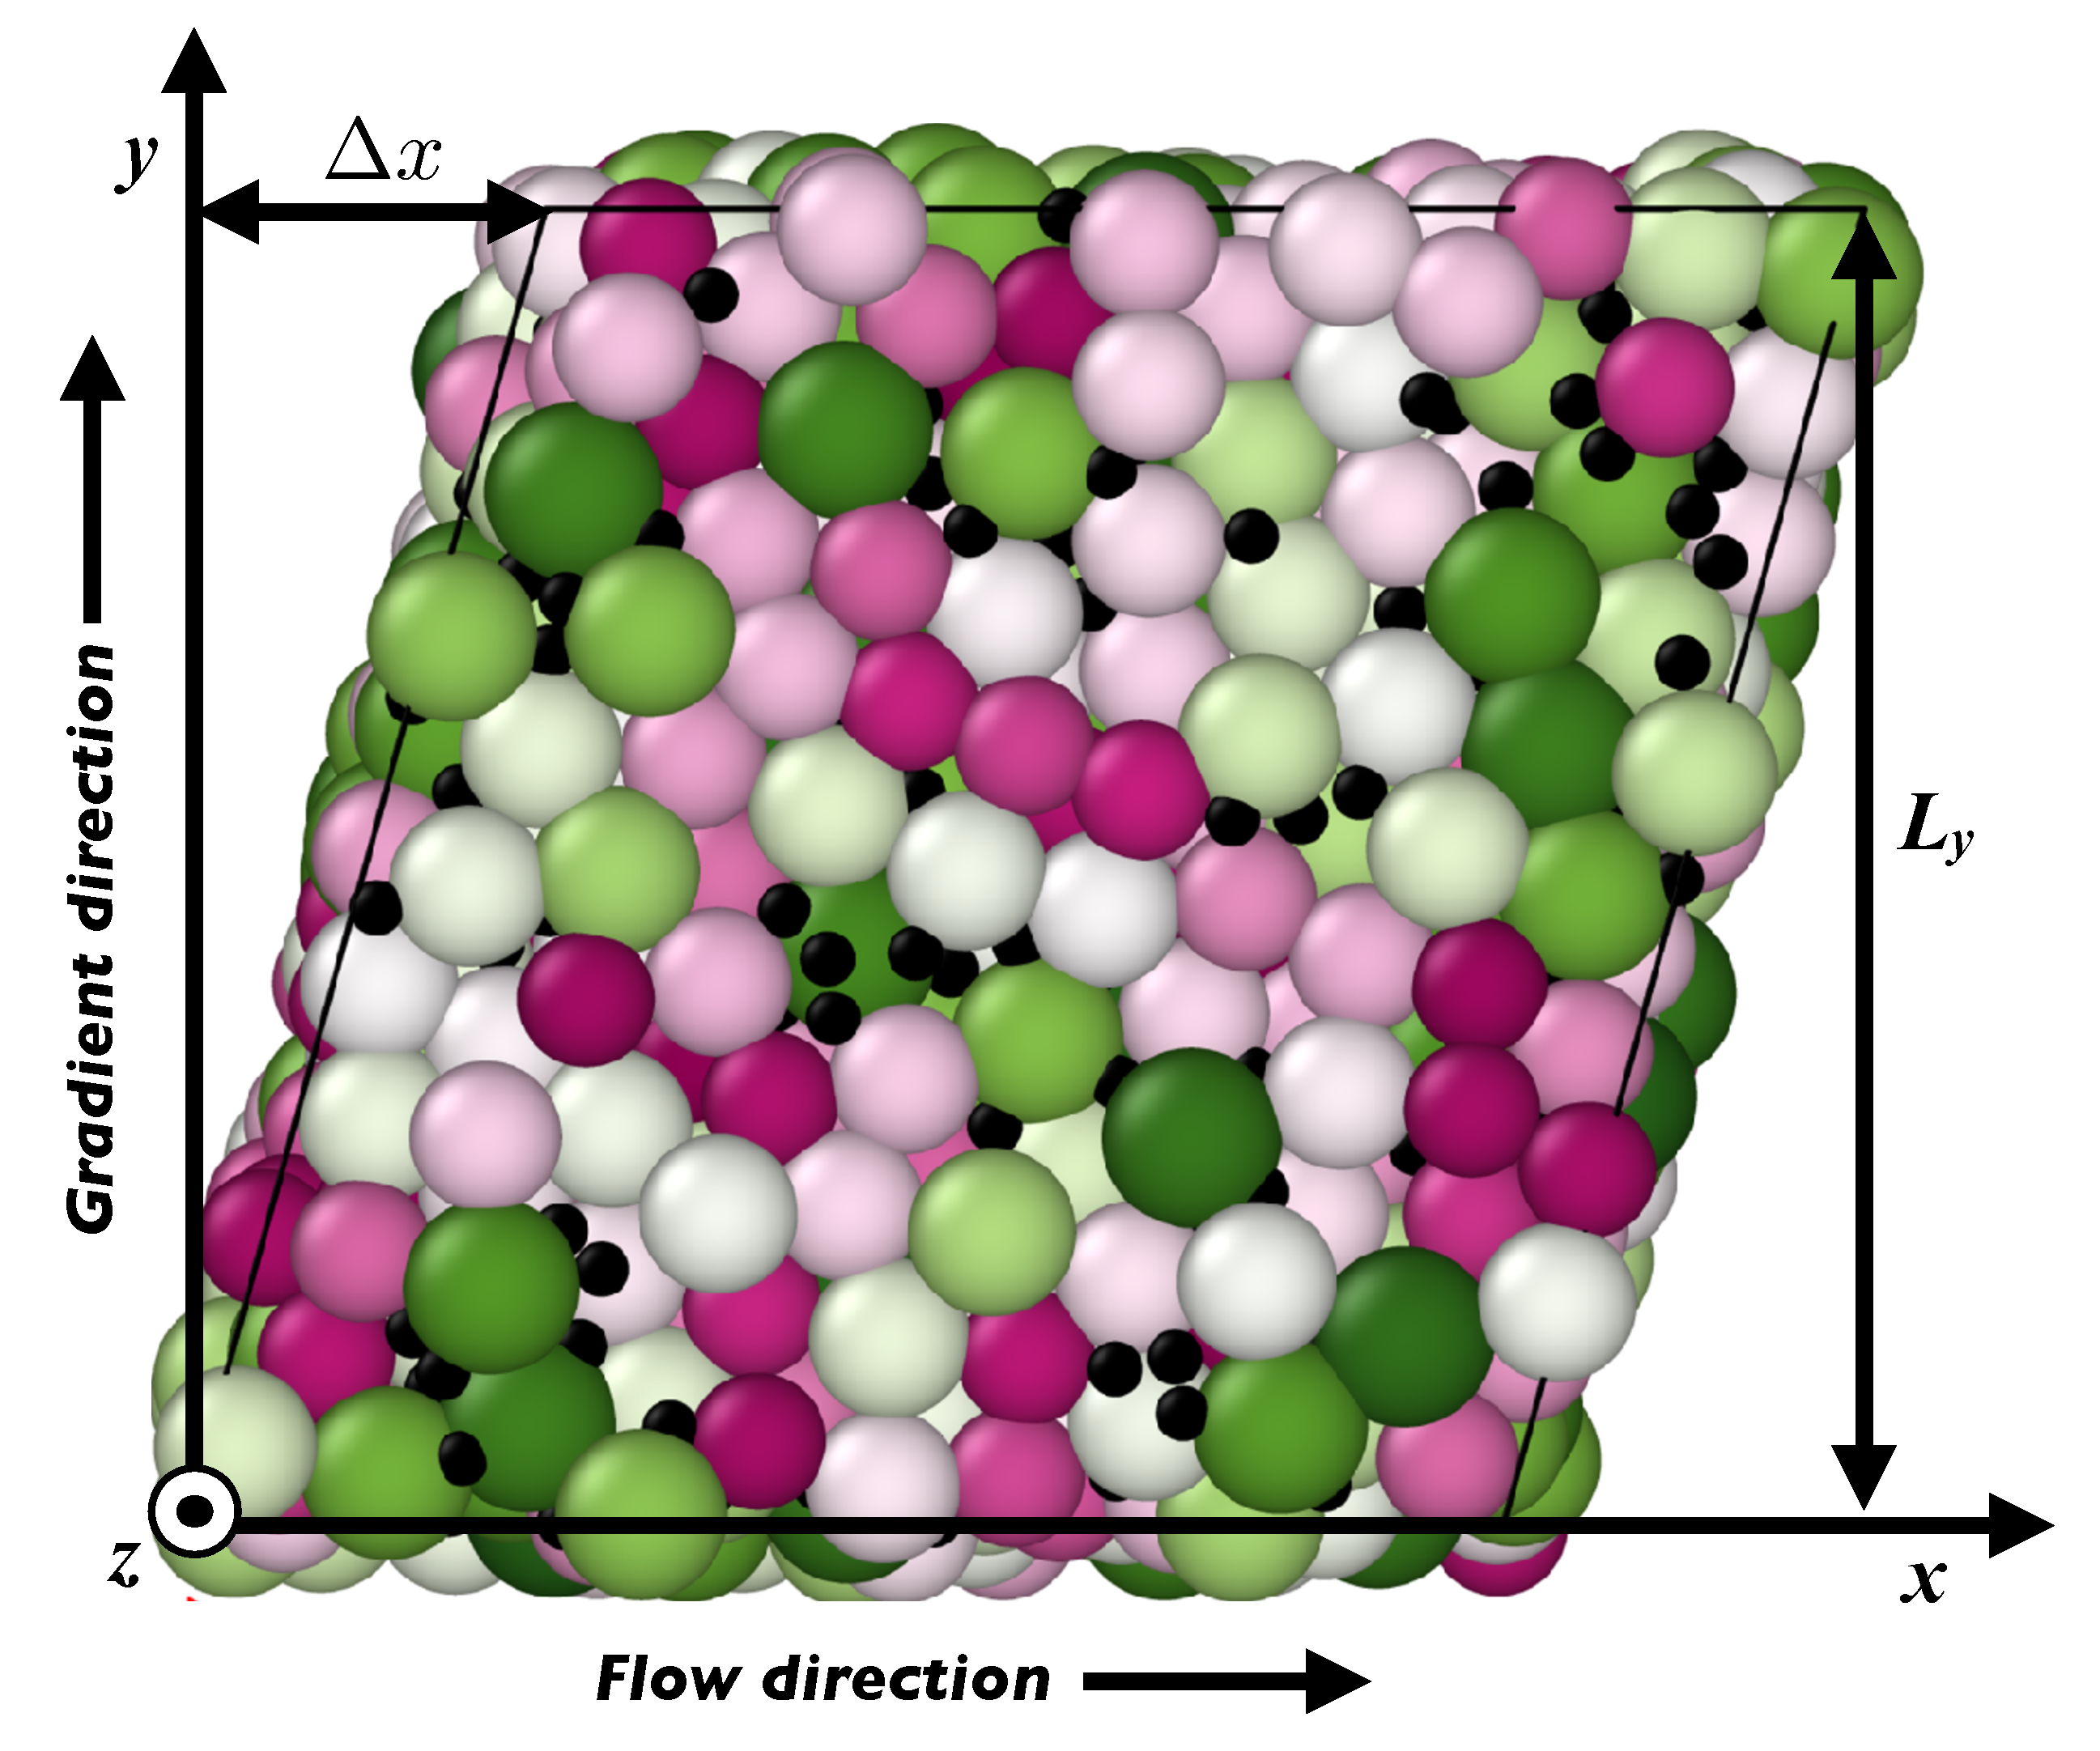
\includegraphics[width=14cm]{figs/couetteFlow.pdf}
	\centering
	\caption[{\em Schematic showing the shear deformation for a planar Couette flow}]{Schematic showing the shear deformation for a planar Couette flow geometry. Here loading is done in the $x$-direction such that $xy$-plane is deformed, resulting in a flow in $x$-direction and gradient of flow velocity in $y$-direction. \label{couetteFlow}}
    \end{figure}
    
    Shear stress $\sigma_{xy}$ is defined as the deforming force $F_{xy}$ (load)  applied parallel to the surface per unit area i.e.,
    \begin{equation}
        \sigma_{xy} = \frac{F_{xy}}{A}
    \end{equation}
    where $A$ is the area of the $xz$-plane of the geometry. Shear strain $\gamma$ is a measure of the deformation of the sample, defined by,
    \begin{equation}
        \gamma = \frac{\Delta x}{L_y}.
    \end{equation}
    
    \begin{figure}[hbt!]
	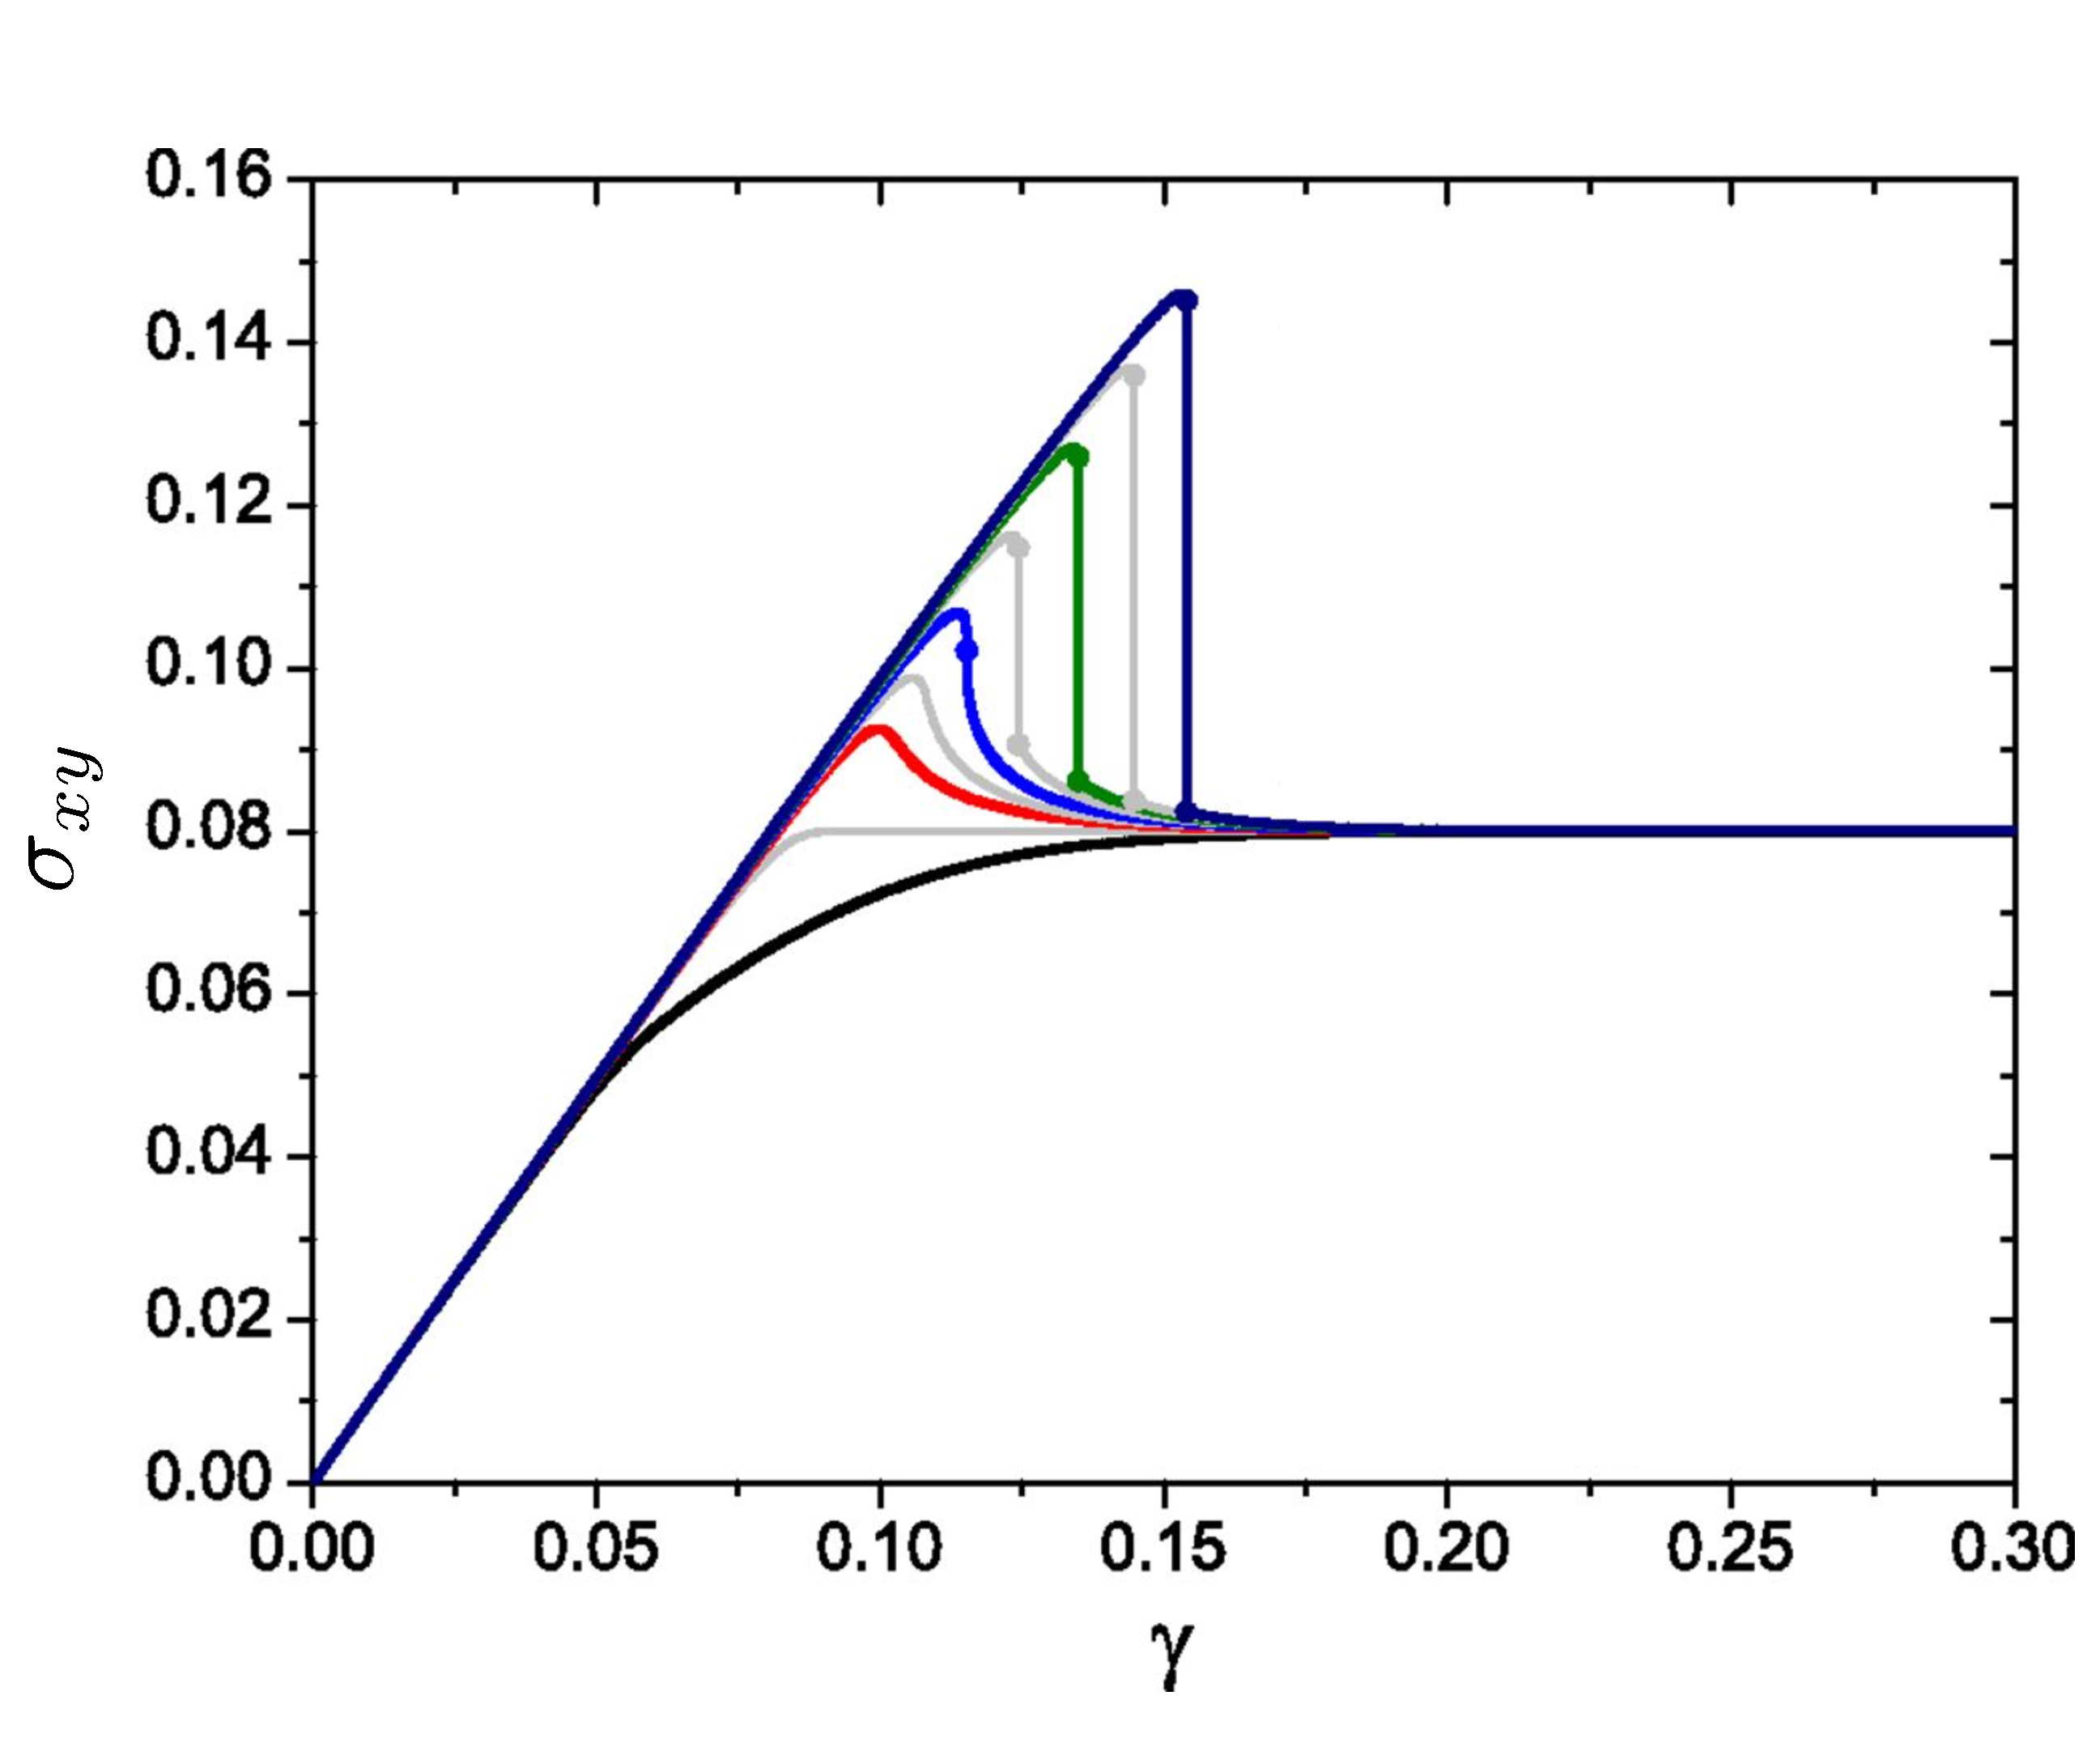
\includegraphics[width=14cm]{figs/fig_stressStrain.pdf}
	\centering
	\caption[{\em Dependence of stress $\sigma_{xy}$ on strain $\gamma$}]{Dependence of stress $\sigma_{xy}$ on strain $\gamma$. Figure adapted from \cite{ozawa2018random}. \label{fig_stressStrain}}
    \end{figure}
    
    In a strain controlled study\footnote{other protocol could be stress controlled, also known as creep} where the system is deformed at a fixed strain rate $\dot{\gamma}$ (stain rate is sometimes loosely spoken as shear rate) such that $\gamma = \dot{\gamma} t$ ($t$ being time here), the typical stress-strain dependence look something similar to as shown in Fig.~\ref{fig_stressStrain}. Here we see, initially, stress $\sigma_{xy}$ increases linearly with strain until a point where it becomes maximum followed by a drop in stress\footnote{This drop could be sharp or extended over a strain window, depending on the type of material brittle or ductile respectively.}. After the drop, the stress becomes gradually steady with strain. So, there are three regimes. The first linear regime is called the elastic branch, where the system behaves like a Hookean solid and the deformation is affine i.e. if the external load is removed within elastic strain window then system returns back to its original undeformed state. At the microscopic scale, all the particle rearrangements are reversible. Also, one defines an elastic modulus $G$ as the ratio of stress to strain, which is actually the slope of the elastic branch.  In the second regime, known as the transient regime, the system starts deviating from the elastic behaviour and microscopic rearrangement of a fraction of particles becomes irreversible i.e., non-affine deformation (plastic deformation). During the plastic deformation, many small zones containing a few particles, known as shear transformation zone (STZ) \cite{falkLanger98}, can be identified which take part in the irreversible plastic rearrangement. In this regime, after the stress overshoot, the system goes to a steady state which is the third regime. This is known as {\em yielding transition} and somewhere close to the overshoot, the yielding point can be identified. In the steady regime, the whole system is fluidized and flows with a steady value with a linear velocity profile.
    
    \begin{figure}[hbt!]
	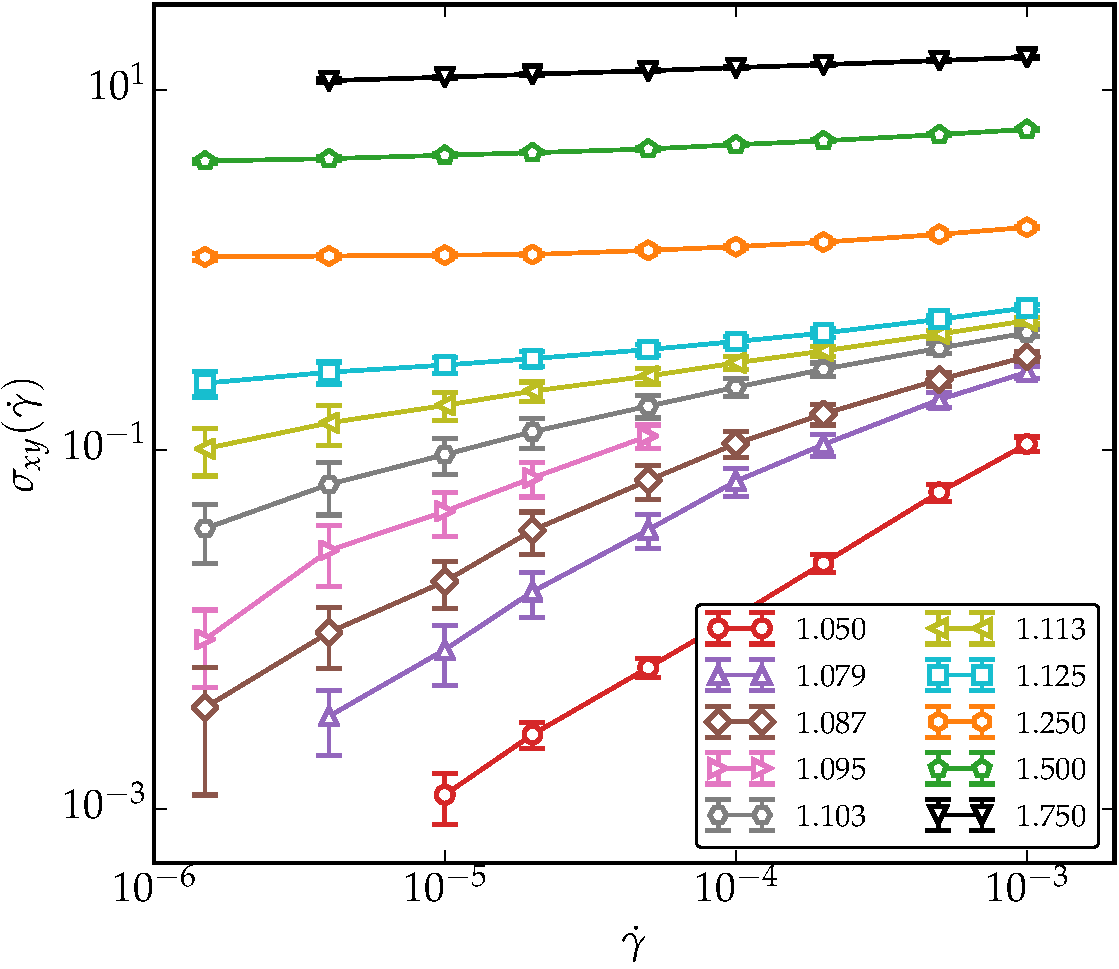
\includegraphics[width=14cm]{figs/fig_stress.pdf}
	\centering
	\caption[{\em Flow curve: dependence of stress on shear rate}]{{\em Flow curve.} Dependence of stress on shear rate for the glass-forming model in \cite{vaibhav2022finite,vaibhav2020response}, at densities varying from small value in liquid state to large value in the glassy state.\label{fig_stress}}
    \end{figure}
    
    In a steady state, the flow behaviour of a material is characterized if the steady stress value is plotted as a function of shear rate, to obtain something known as {\em flow curve}. One such set of curves measured for a glassy liquid, as this forms glass from a supercooled liquid with increasing density, is shown in Fig.~\ref{fig_stress}. Here we can identify different linear and non-linear regimes. The linear regime is exhibited by either a liquid state far from the glass transition point or by supercooled states at a small shear rate window, which contracts as the state moves closer to the glass transition point. Such linear behaviour shown by the liquid is called {\em Newtonian}. For such a case, in the stress-strain curve, we don't observe any overshoot, initially, there is an elastic regime, and then it saturates to a finite value in a steady state. The liquid showing non-linear response is called {\em non-Newtonian liquid}. Supercooled states very close to the glassy state behave non-linearly over a larger window of shear rate and glassy states don't have linear regimes at all. For glassy states, shear stress has a finite value (called dynamic yield stress) at vanishing shear rate, unlike the case for liquid states  where shear stress tends to vanish as shear rate decreases. Materials showing dynamic yield stress are popularly known as {\em yield stress materials} and glasses belongs to this class. For such materials, the flow curves can be described by the {\em Herschel–Bulkley} form given by,
    \begin{equation}
        \sigma = \sigma_0 + k \dot{\gamma}^n
    \end{equation}
    where $\sigma_0$ is the estimation of dynamics yield stress, $k$ and $n$ are constants. For Newtonian liquid, $n=1$ and $\sigma_0 = 0$. We discuss more this aspect in chapter-7.
    
     \begin{figure}[hbt!]
	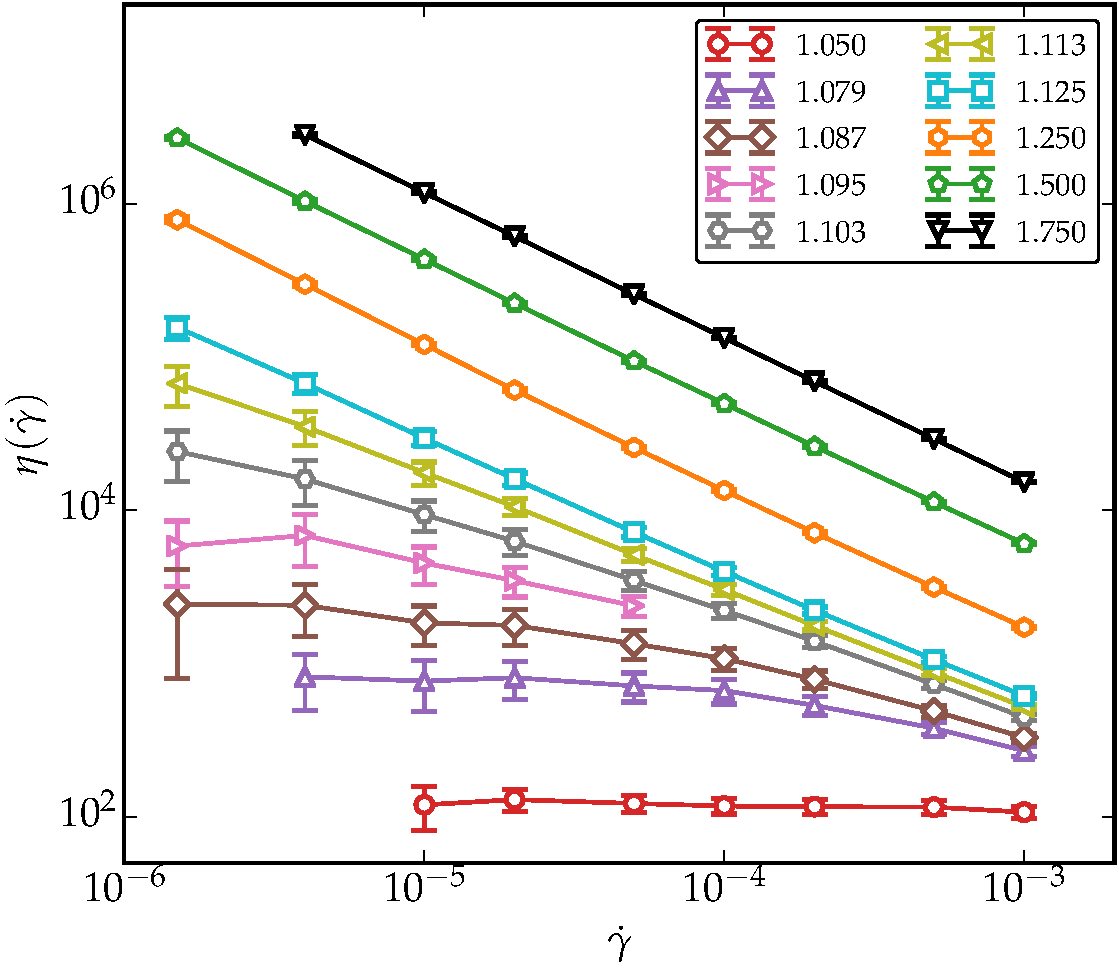
\includegraphics[width=14cm]{figs/fig_viscosity.pdf}
	\centering
	\caption[{\em Dependence of viscosity on shear rate}]{Dependence of viscosity on shear rate for the glass-forming model in \cite{vaibhav2022finite,vaibhav2020response}, at densities varying from small value in liquid state to large value in glassy state.\label{fig_viscosity}}
    \end{figure}
    
    Shear viscosity is defined as the ratio of the stress value to shear rate i.e.,
    \begin{equation}
        \eta = \frac{\sigma_{xy}}{\dot{\gamma}}.
    \end{equation}
    The dependence of steady-state viscosity on shear rate for the data presented in Fig.~\ref{fig_stress} is shown in Fig.~\ref{fig_viscosity}. As it is very clear here, for the liquid far from glass transition, the viscosity is independent of shear rate, behaving as a Newtonian liquid. As the liquid moves closer to the glass transition point in the supercooled state, the behaviour is Newtonian only for very small shear rates \cite{golkia2020}. So, whether the behaviour of liquid is Newtonian or non-Newtonian depends not only on the state of the system i.e., how close the liquid is to the glass transition point but also on the shear rate. As we have mentioned in the previous section, the viscosity of the material increases by several orders of magnitude near the glass transition point. We can see here in Fig.~\ref{fig_viscosity}, the viscosity of the system in high density glassy states is very high even at small shear rates. But, overall the viscosity decreases with the increase in shear rate, this behaviour is known as {\em shear thinning}, common to all glassy systems.
    
    Various theoretical frameworks, e.g. non-local fluidity models \cite{goyon2008spatial}, shear transformation zone (STZ) theory \cite{falkLanger98}, soft glass rheology (SGR) models \cite{sollich1997rheology,sollich1998rheological}, and diverse elastoplastic models \cite{nicolas2018deformation} based on such principles have been proposed and continue to be utilized to develop our understanding of the observed rheological response, discussed above, from a continuum perspective based on the fundamental understanding of the mechanical processes involved. Linking these models to microscopic models is also an important task that has been taken up in recent times.
    
    %%%%%%%%%%%%%%%%%%%%%%%%%%%%%%%%%%%%%%%%%%%%
    \subsection{Shear banding}
    
    \begin{figure}[hbt!]
	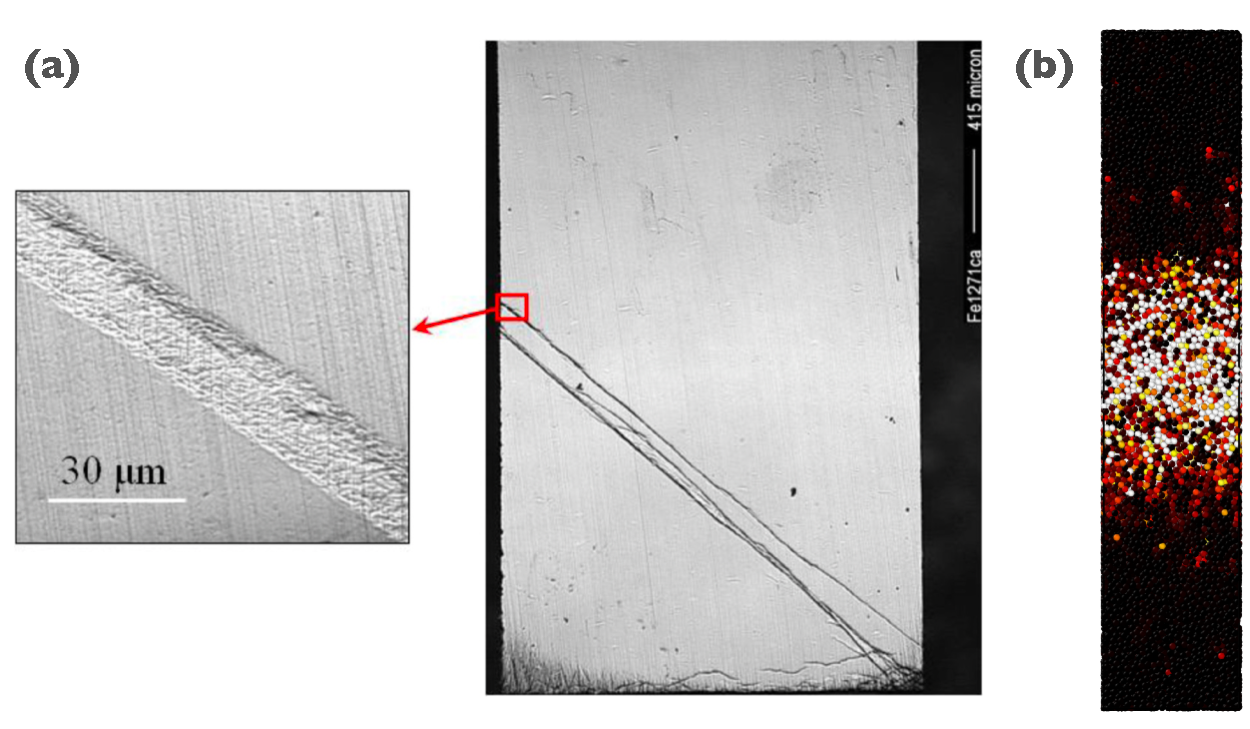
\includegraphics[width=14cm]{figs/shearBand.pdf}
	\centering
	\caption[{\em Shear band formation in glassy system}]{(a) Development of Shear band in nanocrystalline iron grain under a compression protocol \cite{wei2002evolution}. (b) Shear band formed in the fixed shear rate simulation of Kob-Andersen binary Lennard-Jones mixture \cite{kob1995testing}.\label{fig_shearBand}}
    \end{figure}
    
    In many glassy materials,  when stress decays over a small strain window after the stress overshoot, the deformation pattern can be spatially inhomogeneous, forming a band like structure with relatively high mobility known as {\em shear band} \cite{gauravPRE15,golkia2020,anshul17}. The mechanism of formation of shear band in a material is not very clear. It can depend on the preparation protocol of the material \cite{ozawa2018random,ozawa2022rare} and also on the deformation protocol. One hypothesis about the formation of shear band is proposed in terms of percolating cluster of STZ i.e., different plastically deformed regions combine to form shear band \cite{dasgupta2013yield,hassani2019probing}. Another study related to a model metallic glass \cite{gauravPRE15} proposes the formation of shear band as the result of the formation of percolating cluster of mobile regions. The structure i.e., local energy and density inside the bands can be different from the other part of the material \cite{lewandowski2006temperature}. Predicting the location of shear band nucleation has not been completely possible and this is an active area of research. Recently, various machine learning approaches have been attempted for such prediction \cite{fan2022predicting}.
    
    In this thesis in chapter-\ref{chap4}, we can study the shear band formation in the context of an inhomogeneous glass obtained via thermal processing.
    
    %%%%%%%%%%%%%%%%%%%%%%%%%%%%%%%%%%%%%%%%%%%%
    \subsection{Poiseuille flow}\label{PoiseuilleFlow}
    A pressure induced flow through a channel or pipe is called Poiseuille flow which is very common to many natural systems and applications like microfluidic devices, 3D printing, etc, involving glasses. First, let's discuss the hydrodynamic equations based on Navier Stokes equation to understand the predictions of stress profile, velocity profile, and temperature profile in the context of the Poiseuille flow of a Newtonian liquid.
    
    Let's consider an isotropic fluid confined between two parallel plates in the $z$-direction and the particles in the fluid are under the influence of external force ${\bf F_x}$ in the $x$-direction. The equation of motion considering local momentum conservation, can be written as \cite{travis1997departure,travis2000},

    \begin{equation}
    \rho_{m} \frac{d{\bf v}}{dt} = -\nabla {\bf P} + \rho {\bf F_x}
    \end{equation}
    
    where $\rho_m$ is the mass density, ${\bf P}$ is the pressure tensor, $\rho$ is the number density and ${\bf v}$ is the streaming velocity. The above equation is written assuming that the local equilibrium condition holds. Since the fluid is isotropic, the pressure tensor ${\bf P}$ can be split into viscous part $\boldsymbol{\sigma}$ and hydrostatic part ${\bf 1} p$ (${\bf 1}$ is isotropic second rank tensor):
 
    \begin{equation}
     {\bf P} = \boldsymbol{\sigma} + {\bf 1} p.
    \end{equation}
    
    \begin{figure}[hbt!]
	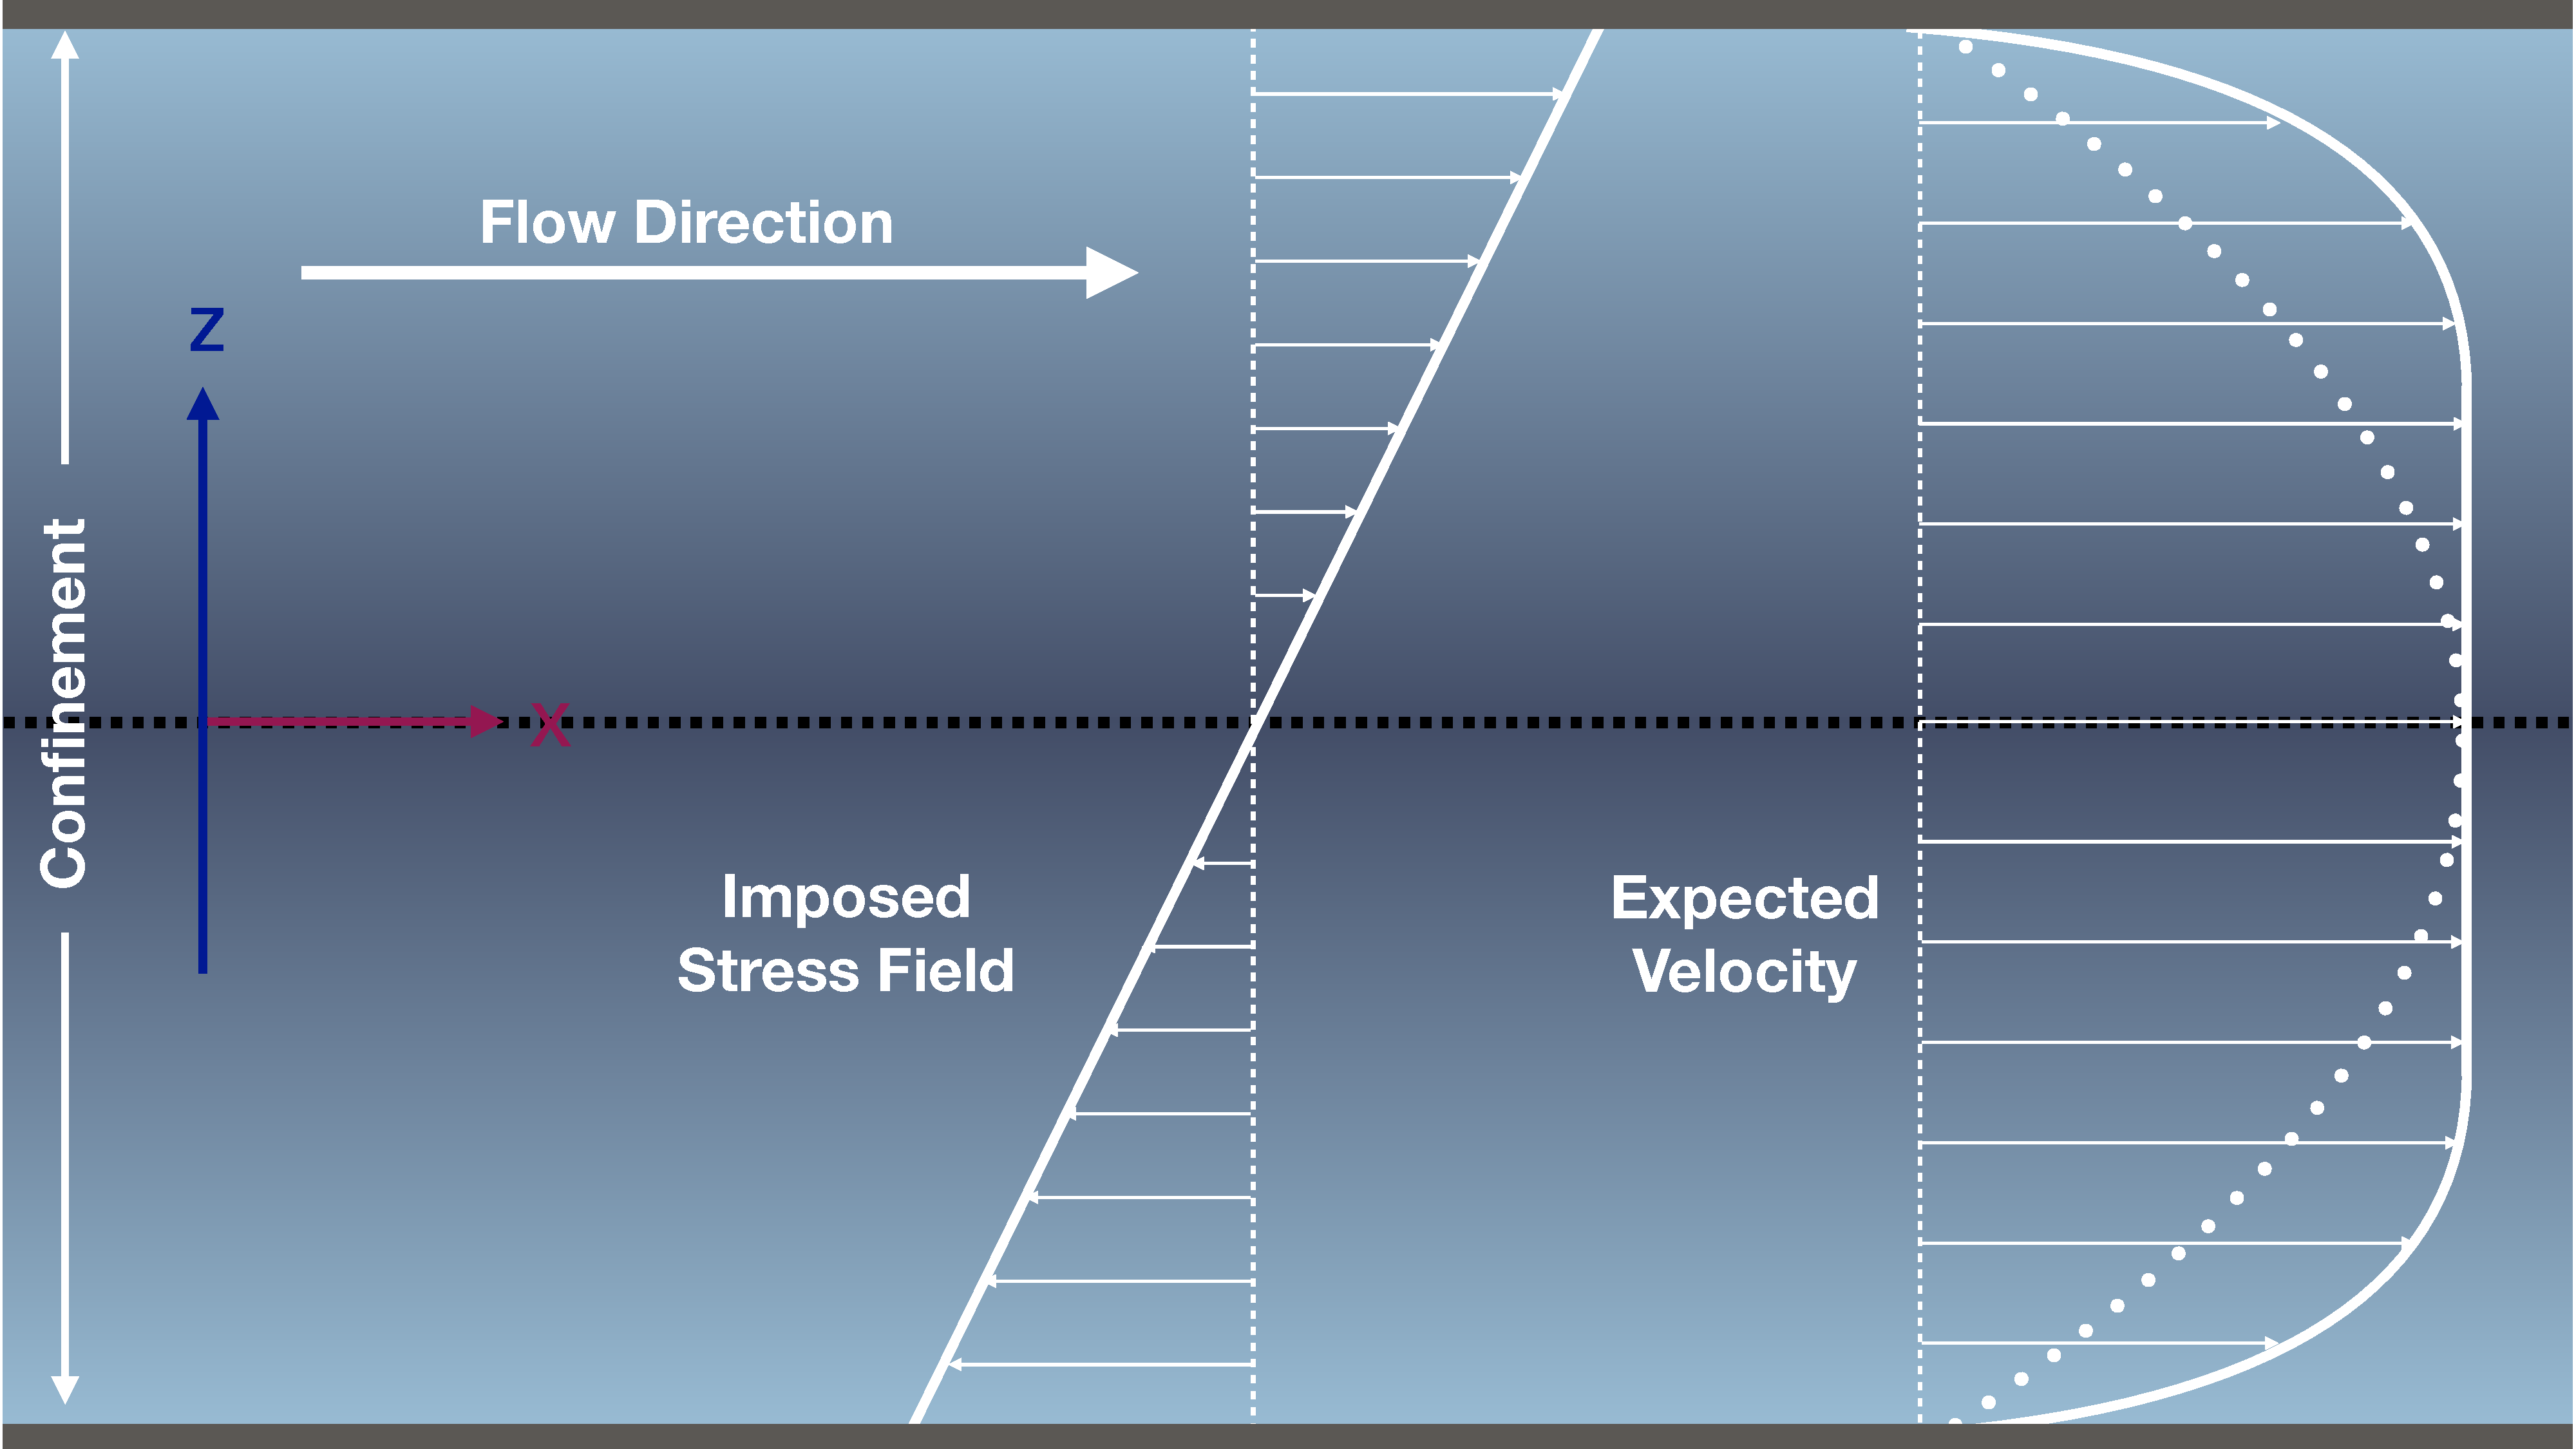
\includegraphics[width=14cm]{figs/poiseuilleFlow.pdf}
	\centering
	\caption[{\em Schematic showing Poiseuille flow}]{{\em Schematic showing Poiseuille flow.} Flow is happening in the $x$-direction and the confinement is in the $z$-direction. This develops linear stress $\sigma_{xz}$ profile. The velocity profile for Newtonian liquid is quadratic (shown with a dotted line) but for yield stress fluid the velocity profile becomes blunt. \label{fig_poiseuille}}
    \end{figure}
 
    For the present setup of Poiseuille flow (as shown in Fig.~\ref{fig_poiseuille}) where the external force on the particles is in the $x$-direction and confinement is in the $z$-direction, the above equation of motion in the steady state is reduced to

    \begin{equation}
    \frac{d\sigma_{xz}(z)}{dz} = \rho F_x.
    \label{stressEq}
    \end{equation}

    If the number density is spatially not varying, the above equation can be integrated to obtain a linear variation of stress:
    $\sigma_{xz}(z) = \rho F_x z$. Also, for a Newtonian liquid, stress $\sigma_{xz}$ is considered linearly varying with the shear rate $dv_x/dz$ i.e.,

    \begin{equation}
    \sigma_{xz}(z) = -\eta(z) \frac{dv_x(z)}{dz}.
    \label{NwtnViscEq}
    \end{equation}
    where $\eta(z)$ is the shear viscosity of the fluid. Now combining eq.\ref{stressEq} and eq.\ref{NwtnViscEq} we get,

    \begin{equation}
    -\frac{d}{dz} \Big[ \eta(z) \frac{dv_x(z)}{dz}\Big] = \rho F_x.
    \end{equation}

    This equation can be solved \cite{travis1997departure,travis2000} to get the spatial variation of velocity, considering a boundary condition and assuming no spatial variation of shear viscosity. If no slip boundary conditions i.e., flow velocity is zero near the boundaries ($v_x(\pm w/2) = 0$), the origin is at the center of the channel and $w$ is the channel width), are considered:

    \begin{equation}
    v_x(z) = - \frac{\rho F_x}{2\eta} \Big( z^2 - \frac{w^2}{4}\Big).
    \end{equation}
    This is the well known quadratic velocity profile for Poiseuille flow.

    Similarly, if the temperature of the flowing fluid in the Poiseuille setup is controlled via walls such that the temperature of the wall is always maintained at $T_0$, the Navier-Stokes equation for energy in steady state can be written \cite{todd1997temperature}:

    \begin{equation}
    \frac{dJ_{Qz}(z)}{dz} + \sigma_{xz}(z) \frac{dv_x(z)}{dz} = 0.
    \end{equation}
    Here $J_{Qz}$ is the steady heat flux in the $z$-direction, which can be written in terms of temperature gradient using Fourier's law as ($\lambda$ as the thermal conductivity of the fluid): $J_{Qz} = -\lambda(z) \frac{dT(z)}{dz}$. Also, we use eq.\ref{NwtnViscEq} then the above energy equation can be simplified,

    \begin{equation}
    -\frac{d}{dz} \Bigg[ \lambda(z) \frac{dT(z)}{dz} \Bigg] - \eta(z) \Big( \frac{dv_x(z)}{dz} \Big)^2.
    \end{equation}

    Again, assuming no spatial variation of thermal conductivity and shear viscosity, and considering the boundary condition $T(\pm w/2) = T_0$, the above equation can be solved to obtain the spatial variation of temperature:

    \begin{equation}
    T(z)=T_0 + A(\rho_0{F_x}w^2)^2[1-(2z/w)^4].
    \end{equation}

    Here $A$ is a parameter depending on the thermal conductivity and shear viscosity of the fluid.
    
    As we can see here, stress varies linearly in the channel, velocity has quadratic variation while temperature has quartic variation. All these variations have been obtained for incompressible Newtonian liquids. But the behaviour of these quantities is expected to be different when the fluid is Non-Newtonian. Glass is a very special type of non-Newtonian fluid that has finite yield stress i.e., glass flows only if stress is above a threshold. Since here in Poiseuille flow, stress varies from zero to a maximum value as we go away from the center of the channel, so for glassy fluid, it is expected that there should be no flow in the center of the channel. Therefore velocity profiles will be blunt at the centre, as shown in Fig.~\ref{fig_poiseuille}. But spatiotemporal correlations of the glass make the situation complicated and the velocity profile can become rounded at the center \cite{goyon2008spatial}. We discuss this aspect in detail in chapter-\ref{chap5}. 
    
\section{Organisation of the thesis}
This thesis is organized into seven chapters. In this first chapter, we have introduced the title of the thesis i.e., "{\em Thermo-mechanical response of glassy systems}". Also, we have briefly discussed some relevant properties of the glass-forming system in this chapter, along with the basic background regarding observables that characterize their structure and dynamics. Further, a general discussion has been presented about the different approaches that are employed to study the thermal and mechanical response of glasses.

In Chapter-\ref{chap2}, we have discussed the numerical tools that have been used to perform computer simulations in the rest of the chapters. In particular, we discuss the method of molecular dynamics (MD) simulations in the context of equilibrium and nonequilibrium systems. The basic implementation strategy, boundary conditions, thermostatting technique, etc. are discussed for MD. Also, the technique of hybrid swap Monte Carlo- Molecular dynamics is discussed, which we have used in Chapter-\ref{chap6} to equilibrate a binary mixture at higher densities. At the end of the chapter, details related to different glass-forming models used in various studies in this thesis, are presented.

We have studied the thermal response of a glass-forming model system using large-scale molecular dynamics simulation in Chapter-\ref{chap3}. The system is studied at first in the supercooled regime to understand the coupling of heat and mass transport, resulting because of an externally applied temperature gradient. Also, numerical results are presented to explore the validity of linear response. The response in the glassy regime is also studied. At the end of the chapter, we study the response of a glassy sample to a time pulse of thermal gradient.

The study related to the response of the glass to a thermal gradient pulse, performed in Chapter-\ref{chap3} is extended in Chapter-\ref{chap4}, by studying the mechanical response of the systems generated via the application of the thermal gradient. Here, we apply the thermal gradient pulse by varying the strength of the gradient and their exposure time to prepare glassy samples with different degrees of spatial heterogeneity in density, concentration and local potential energy. The mechanical response of these inhomogeneous glassy samples is studied by imposing a fixed shear rate. The macroscopic shear response is measured in terms of the temporal evolution of shear stress and average potential energy. Further, we try to understand the role of heterogeneity in the mechanical failure of these thermally processed samples by observing shear band formation.

In Chapter-\ref{chap5}, we study the Poiseuille flow of a glassy liquid, where the temperature of the flowing liquid is controlled via two different mechanisms: one via the confining walls maintained at the target temperature and the other by applying a thermostat directly to fluid keeping the wall frozen. We compare the rheological consequences in transient and steady states, in the two different thermalization protocols.

The last study in this thesis, reported in Chapter-\ref{chap6}, is focused on a glass-forming binary mixture with large size ratio. At first, we study the structural and dynamical properties of the mixture, specifically focused on the collective interdiffusion process. Then, this is followed by a detailed exploration of rheological properties, to understand how rigidity sets in such mixtures. Further, we provide a microscopic analysis of the observed macroscopic shear responses.

Finally, the thesis is concluded in Chapter-\ref{chap7} with a summary of the main results studied here, followed by a discussion on the future directions in which the various results of this thesis can be extended to establish new milestones.

